\documentclass[9pt,nocopyrightspace,preprint]{sigplanconf}
% preprint for dates
\bibliographystyle{plainnat}
\usepackage{amsmath,amsthm}
\usepackage{listings}
\usepackage{tikz}
\usepackage{subfigure}
\usepackage{multirow}
\usepackage{pgfplots}
\usepackage{booktabs}
\usepackage{dcolumn}
\usepackage{cancel}
\usepackage{multirow}
\usepackage{ifmtarg}
\usepackage{url}
\usepackage{bcprules}
\usepackage{verbatim}
\usepackage{graphicx}
\usepackage{chngpage}

%\newcommand{\infrule}[2]{\displaystyle\frac{\displaystyle\strut{#1}}{\displaystyle\strut {#2}}}
\newcommand{\deref}{\ast}
\newcommand{\rread}[1]{\mbox{\em Read}(#1)}
\newcommand{\rwrite}[1]{\mbox{\em Write}(#1)}
\newcommand{\lca}[2]{#1 \sqcup #2}
\newcommand{\rleq}{\leq}
\newcommand{\interval}[1]{\mbox{\em interval}(#1)}
\newcommand{\context}[1]{\mbox{\em context}(#1)}
\newtheorem{theorem}{Theorem} 
\newtheorem{lemma}[theorem]{Lemma}
\newcommand{\texcomment}[1]{}

\begin{document}

%\title{A Type System for Structured Aliasing in Parallel Programs}
\title{Supporting Dynamic Data Partitioning in Parallel Programs}
%\title{Scalable and Safe Parallelism using Logical Regions}
\authorinfo{Sean Treichler \and Michael Bauer \and Alex Aiken}{Stanford University}{\{sjt,mebauer,aiken\}@cs.stanford.edu}
%\authorinfo{Sean Treichler}{Stanford Unviersity}{sjt@cs.stanford.edu}
%\authorinfo{Michael Bauer}{Stanford University}{mebauer@cs.stanford.edu}
%\authorinfo{Alex Aiken}{Stanford University}{aiken@cs.stanford.edu}
\maketitle

\begin{abstract}
Many distributed-memory parallel applications dynamically partition 
data, but current language designs either 
require fully static partitioning or rely on expensive dynamic checks.
We describe Legion, a programming system with a combination
of language features and static and dynamic checks to support 
dynamic data partitions with minimal overhead.
We describe the novel aspects of the Legion design, prove the soundness of the Legion type system,
 and show Legion type checking improves performance by up to 71\% by eliding provably
safe memory checks.  Furthermore, we show how the language design and type safety
enables a hierarchical, distributed runtime scheduling algorithm, and how
a system of data coherence annotations improves expressivity without compromising
soundness. We report results for three real-world applications running
on distributed memory machines, achieving up to 62.5X speedup on 96 GPUs 
on the Keeneland supercomputer.
%Legion is a programming model that introduces
%{\em logical regions} as a mechanism for targeting large heterogeneous machines 
%with complex memory hierarchies.  Logical regions are first-class 
%values in Legion, and programmers may {\em partition} regions in multiple different
%ways into subregions.  We present
%a type system with privileges and coherence properties for reasoning about logical regions.  
%We prove the soundness of the type system and use it to show
%that all memory accesses in Legion are safe.  Furthermore, we prove that
%type soundness enables a scalable, hierarchical
%scheduling algorithm for Legion programs.  We show that an implementation of the type checker
%for Legion programs improves performance up to 71\% by eliding
%memory checks the type system proves safe.  We also demonstrate that an implementation of the Legion 
%runtime based on the hierarchical scheduling algorithm scales well for
%three real-world applications.


%Limit is 12 pages, including bibliography and appendices.
%Deadlines: \\

%\begin{tabular}{ll}
%Paper registration & July 7, 2012 3:59am PDT \\
%Paper submission & July 11, 2012 3:59am PDT \\
%Author response & September 10 - September 13, 2012 \\
%Author notification & October 1, 2012
%\end{tabular}
\end{abstract}



\section{Introduction}
\label{sec:intro}

Machine architecture, particularly at the high
performance end of the spectrum, has recently undergone a revolution.  The
latest supercomputers are now composed of heterogeneous processors
and deep memory hierarchies.  Current programming systems for these
machines have elaborate features for describing parallelism, but 
few abstractions for describing the organization of data.  However, as 
distributed memory machines increase in complexity,
reasoning about the organization of program data will be imperative
for supporting the management of parallelism and the movement of data
through the memory hierarchy.

%Consequently, the burden of managing
%the correctness of parallel computations and movement of data
%through the memory hierarchy is placed on the programmer.

%However,
%these systems relegate to the programmer the responsibility for:
%\begin{itemize}
%\item the correctness of their parallel declarations
%\item the movement and placement of data in the memory hierarchy
%\end{itemize}
%Coupled with the complexity of these machines, this places a heavy
%burden on the programmer.  The reason that the programmer must bear
%this load is because current programming systems have few or no
%insights into properties of program data (e.g. locality and independence).  
%To enable more efficient programming of this class of machines we 
%need programming systems capable of reasoning both statically and dynamically
%about the structure of program data.

Previous work has explored two approaches for describing the organization of data
in distributed memory programs.
One class of work uses fully static analyses with no runtime overhead, but 
disallows potential data aliasing to make the analysis tractable, limiting expressivity.
Two recent examples, Sequoia \cite{Fatahalian06} and 
Deterministic Parallel Java (DPJ) \cite{Bocchino09}, each provide a 
mechanism to statically partition the heap.
% into a tree of collections of data.
The two designs are different in many aspects, but agree that there is
a single tree-shaped partitioning of data that must be checked statically 
(see Section~\ref{sec:related}).  The second approach permits data
aliasing, allowing greater expressivity, but uses fully dynamic analyses of
program execution to detect aliasing and guarantee correct results.
This approach incurs significant runtime overhead and requires 
centralized control logic that is difficult to scale to distributed 
memory machines; examples include transactional memory \cite{Harris05} 
and thread-level speculation \cite{Steffan00}.

Our own experience writing high-performance applications
using the current industry standard mix of MPI, shared-memory
threads, and CUDA has taught us that a
single, static data partitioning is often insufficient.  In many cases, the
best way to partition data is often a function of the data
itself---i.e., the partitions must be dynamically computed and cannot be statically described.
Furthermore, applications often need multiple, simultaneous partitions of
the same data, which introduces aliasing.

In this work, we present the static and dynamic semantics of Legion \cite{Legion12},
a parallel programming model that supports multiple, dynamic data partitions and is
able to efficiently reason about potential aliasing.
Legion's {\em logical regions} are an abstraction capturing {\em locality} 
(data that will be used together, and therefore should be colocated) 
and {\em independence} (disjoint data that may be operated on in parallel).  
Logical regions have properties that allow programmers to communicate information
about the structure of program data to the Legion implementation:
\begin{itemize}
\item  logical regions are first-class values in Legion
and may be dynamically allocated and stored in data structures;

\item logical regions can be dynamically {\em partitioned} into {\em subregions}; 
the programmer can express arbitrary partitions of regions;

\item  a logical region may be dynamically partitioned in multiple different ways;
subregions from multiple partitions may include the same data, introducing 
aliasing\footnote{Thus
  the term {\em logical} regions: language-level regions
  name sets of data but do not imply a physical layout or placement in
  the memory hierarchy. A separate system of {\em physical regions} at
  runtime holds copies of data in the language-level logical regions
  \cite{Legion12}.}.

%\item {\em privilege} and {\em coherence} properties that
%describe how a logical region's data may be used by computations (explained below).
\end{itemize}

%Both dynamically computed partitions
%and simultaneous partitions of the same data introduce the possibility
%of {\em aliasing}---distinct regions may have overlapping data.

While data in Legion is organized in a hierarchy of logical regions,
computation is organized in a hierarchy of tasks.  Logical regions and tasks interact
through a system of {\em privileges} that specify which operations (read, write, or reduce)
a task (or any of its subtasks) may perform on each logical region argument.  
%Tasks can only access logical regions for which they 
%possess privileges.  
%Tasks acquire privileges from their calling task
%or by creating new logical regions.  A key restriction is that 
%a sub-task can only be passed a subset of the privileges of its parent task.  

%Through multiple partitions of a logical region, a given datum may
%belong to multiple different regions.  

To support additional parallelism in the presence of aliased data,
Legion provides {\em coherence} modes at the granularity of regions,
which allow relaxed constraints on task execution order, even
in cases where tasks access the same region.  The programmer may
specify that tasks conflicting on a region run in
program order (the default), {\em atomically} with respect to each
other, or even {\em simultaneously} if the application has alternative
methods for ensuring determinism or can tolerate non-deterministic
behavior in that region.

%To guarantee the safety and correctness of programs, Legion relies on
%a combination of static and dynamic analysis based on the privilege
%and coherence systems.  
%To efficiently guarantee the safety and
%correctness of programs using first-class regions,
%privilege and coherence properties in the presence of arbitrary region
%aliasing, Legion relies on a combination of static and
%dynamic checks.  
The critical feature in Legion that makes static analysis tractable
and dynamic analysis efficient in the presence of potential aliasing is logical regions.
Alias analysis is a very hard static analysis problem, but is both easy and
inexpensive if done dynamically at the granularity of logical regions instead
of individual memory locations; similarly
checks on individual memory accesses are expensive if done dynamically, but
cheap if done statically within the context of local logical region privileges.
%A key theme that runs through the design is that 
%alias analysis is a very hard static analysis problem, but is both easy and
%inexpensive if done dynamically at the granularity of regions instead of individual
%heap locations, while checks that must be done on individual values are only
%cheap if done statically.  
Explicating and evaluating the design of Legion's
static and dynamic semantics is the topic of this paper, 
%and its implications are the topics of this paper,
which we present as a series of contributions:
\begin{itemize}
\item We present a type system for {\em Core Legion} programs that statically
  verifies the safety of individual pointers and region
  privileges at task call boundaries (Section~\ref{subsec:coretypes}).
%  A subtle issue arises in checking privileges when regions are
%  stored in and later retrieved from heap data structures.  The type
%  system provides enough static information that the Legion runtime
%  can leverage its dynamic information about region aliasing to
%  perform dynamic privilege checks guaranteeing safety.

\item We present a novel parallel operational semantics for Core Legion.
 This semantics is compositional,
  hierarchical, and asynchronous, reflecting the way such programs
  actually execute on the hardware.  The semantics also
  models conflicting memory operations between tasks in cases of relaxed
  coherence, making explicit the boundary between deterministic and
  possible non-deterministic behavior (Section~\ref{subsec:opsemantics}).

\item We prove the soundness of Legion's static type and privilege system (Section~\ref{sec:soundness}).


\item We use soundness of the type system to prove the soundness of
  Legion's region coherence modes (Section~\ref{sec:coherence}).


\item Again using the soundness of the type system,  we show that if expressions $e_1$ and $e_2$ 
are {\em non-interfering} (can be executed in parallel), then subexpressions
$e_1'$ of $e_1$ and $e_2'$ of $e_2$ are also non-interfering (Section~\ref{sec:scheduling}).  
This result is the basis
for a hierarchical, distributed scheduler in the Legion implementation which is crucial for high performance
on the target class of machines.
%  any form of centralized scheduling would be a bottleneck because of the
%large communication latencies in the target class of machines.
%; on the target class of machines, any centralized
%scheduler would be a serious bottleneck.

\item We give experimental evidence that supports the Legion design choices.  On three
  real-world applications, we show that dynamic region pointer checks
  would be expensive, justifying checking this aspect of the type
  system statically.  We also show that the cost of region aliasing
  checks is low, showing that an expressive and dynamic
  language with aliasing is compatible with both high
  performance and safety (Section~\ref{sec:evaluation}).

\end{itemize}






%The crucial aspect of this result is that the tasks $t_1$ and $t_2$ only 
%need be non-interfering instead of non-aliased.  Thus, through a combination
%of static and dynamic analysis, our privilge type system and coherence system
%enable us to implement a hierarchical, distributed scheduling algorithm even
%in the presence of aliasing introduced by the need for dynamic descriptions of
%data via first-class logical regions.  
%All of this is possible only because
%our programming system supports an abstraction for understanding the structure
%of program data.



%The important difference between Legion and the more static approaches
%is that Legion allows region aliasing, but does so in a structured way that minimizes
%runtime overheads.  
%The key observation is that static alias analysis is hard, but dynamic 
%alias analysis is very easy and relatively cheap when done at the granularity 
%of regions instead of individual heap locations.  
%Thus, Legion falls between fully static systems, such as
%Sequoia and DPJ, and fully dynamic approaches such as transactional
%memory.  
%Legion still has a significant static component; in
%particular, the required privileges for function calls
%and region
%pointer dereferences are checked statically.  The dynamic alias checks
%for independence are done at the granularity of regions and one check 
%on a region
%often serves to prove the independence of many subsequent uses of that region.
%In contrast, because transactional memory has no mechanism
%for grouping heap data into larger collections, it must test the
%overlap between two sets of data on each individual memory location, which is
%significantly more expensive.



%which makes it difficult 
%to statically determine which computations can be run in parallel.  
%One approach is to outlaw aliasing which allows for a static analysis
%to discover all available parallelism and schedule it entirely at
%compile-time, avoiding any runtime overhead.  Languages such as
%Sequoia and DPJ take this approach and allow only a single static partition of any region 
%to eliminate region aliasing, at some cost in expressiveness.



%While many programming systems for
%these machines have intricate features for describing parallelism,
%few have any abstractions for capturing properties of a program's data (e.g.
%independence and locality).  Understanding the structure of a program's data
%is critical for allowing programming systems to validate/discover
%parallelism or support placement of data in the memory hierarchy.  
%The few programming systems that do support data abstraction 
%features\cite{Fatahalian06,Bocchino09} permit only
%statically analyzable abstractions which restrict expressivity.  We
%present a type system for Legion\cite{Legion12}, a programming model
%that permits both static and dynamic descriptions of the structure of 
%program data.  Despite the dual nature of Legion, our type system allows us 
%to statically prove several useful properties about the structure and usage 
%of data in Legion programs.  We show how to leverage these properties 
%to enable a scalable, hierarchical scheduling algorithm based on a 
%dynamic analysis of program data.

%complex hierarchies of many different
%kinds of computing technologies: networks of nodes at the top level,
%multiple chips per node, multiple cores within a chip, and, 
%recently, multiple accelerators (usually GPUs) per node, which 
%can themselves be further decomposed.  We present the operational and static
%semantics of Legion\cite{Legion12}, a programming model targeted at providing an
%appropriate level of abstraction for programming such machines, one
%that is both sufficiently high-level to be portable while still
%exposing aspects that are crucial to performance. 

%The primary abstraction for capturing the structure of data in Legion is {\em logical regions}. Logical
%regions express {\em locality} (data that will be used together, and therefore should be colocated) 
%and {\em independence} (disjoint data that may be operated on in parallel).
%Legion programs organize data into a forest of logical regions.  Logical regions can be
%recursively partitioned into sub-regions.  

%In Legion data is organized in a hierarchy of {\em regions}
%and subregions while computation is organized in a hierarchy of {\em
%tasks} and subtasks operating on regions.  Regions and tasks interact
%through a static system of {\em region privileges} specifying 
%operations a task may perform on a region argument (read,
%write, or reduce) and  {\em region coherence} annotations that
%express what other tasks may do concurrently with
%the region (exclusive, atomic, or simultaneous).  We prove the
%soundness of the privileges and coherence system and use these two
%results to prove a third result: if two {\em siblings} (tasks that
%have the same immediate parent task) $t_1$ and $t_2$ are 
%{\em non-interfering} (have no ordering requirements for correctness), 
%then the any descendant of $t_1$ in the task hierarchy is non-interfering
%with any descendant of $t_2$.  This theorem is the basis for correct distributed
%task scheduling in a Legion implementation, which is crucial for
%performance; a centralized scheduler would be a bottleneck
%because of the large communication latencies in the target
%class of machines.


% Putting this here so that we can get the code in a good place
% Moving this to the circuit example section since it fits better there
% and some of this is redundant
%Legion's execution model is that by default, a program's semantics is
%its meaning as a sequential program, which we refer to as the {\em
%program order} execution.  While the
%implementation is not our focus here, if two functions use
%disjoint data (because all of the regions they use are disjoint), then
%Legion may execute them simultaneously.  Also like DPJ,
%Legion has a system of {\em privileges} ({\em read}, {\em write}, and
%{\em reduce}) on regions and an orthogonal system of region {\em
%coherence} modes ({\em excl}, {\em atomic}, and {\em simultaneous})
%that increase the number of situations in which functions can be
%executed in parallel.

%The rest of the paper is organized as follows.
%We begin in Section~\ref{sec:example} with an example program that illustrates
%a typical style of programming in Legion and motivates the need for multiple, dynamically computed partitions of
%a region that introduce aliased data.  We define Core Legion, a small language suitable 
%for our formal development, in Section~\ref{sec:legioncore}.
%Finally, Section~\ref{sec:related} discusses the most closely related work and
%Section~\ref{sect:conclusion} concludes.


  













\section{Circuit Example}
\label{sec:example}

Listing~\ref{lst:circuit_ex} shows code for a
circuit simulation written in the core Legion language introduced in
Section~\ref{sec:legioncore} (with one exception described below).  The
circuit simulation takes as input a large graph of circuit elements and wires
connecting the elements.  To perform the simulation in parallel the graph
is partitioned into pieces.  After partitioning
the graph the simulation is run for a number of time steps.  Each time step
consists of three phases: calculating the current on each wire, distributing
charge to the nodes to which each wire is connected, and updating the voltage
of each node.

The top level function in the application is {\tt simulate\_circuit} (line 15).  The {\tt simulate\_circuit} 
function is parameterized on the regions {\tt rl}, {\tt rw}, and {\tt rn} (line 15) which 
implies that the when the function is invoked it must have privileges for the regions 
bound to those parameters.  Furthermore, these privileges must be for both reading 
and writing these regions (line 17).  The only logical regions which {\tt simulate\_circuit} will 
be allowed to access are these regions and their logical subregions.  This property will be 
enforced by the type system introduced in Section~\ref{sec:legioncore}.  {\tt simulate\_circuit}
takes pointers to the lists of nodes and wires that describe the graph.  The nodes
are stored in the {\tt rn} region while wires are stored in the {\tt rw} region.  The
lists live in the {\tt rl} region.  

The first step in {\tt simulate\_circuit} is to partition the graph into pieces.  Partitioning
is done by constructing {\em colorings} using the {\tt color\_circuit} function (line 18-19).  A
coloring is a mapping from region elements to colors with each color corresponding to a new subregion
to be created.  The algorithm for performing a coloring is an application specific decision made by 
the programmer.  Note, that in the case of circuit, it would be impossible to
pick a single static partitioning scheme that would do well for all graphs.  Dynamic partitioning
provides the programmer the flexibility to make partitioning decisions based on input data.

The {\tt color\_circuit} function returns three colorings.  The first coloring is a total 
coloring that maps each node in the graph the piece that owns it.  The third coloring is a total
coloring that maps each wire in the graph to a piece which owns on of its nodes.  The second coloring captures a
different property of the graph: those nodes which must be shared between different pieces of the
graph to perform computations in parallel.  These are often referred to as {\em ghost nodes}.  We
describe how ghost node regions are used in conjunction with the owned nodes later.
Note that its possible some ghost nodes are shared between multiple pieces, and can be colored multiple ways. 
The second coloring is referred to as a {\em multicoloring} because it might map the same element
to multiple colors.

After creating the colorings, the application partitions the region into {\em subregions} based on 
the colorings (lines 21-25).  For simplicity, our example only partitions the circuit into two pieces.  Lines
21 and 23 create two different partitions with two different subregions of the {\tt rn} region.  The first partition is
{\em disjoint} because it is based on a coloring while the second partition is {\em aliased}
because it is based on a multicoloring which does not imply disjointness of subregions.  While 
aliased partitions based on multicolorings are not a part of core Legion described in Section~\ref{sec:legioncore}, 
they are functionally equivalent to creating single partitions for each color in the multicoloring.

Disjoint partitions introduce
disjointness constraints into the static environment indicating that all the subregions in the partition are 
disjoint (e.g. {\tt rn0}$*${\tt rn1} on line 21 says {\tt rn0} is disjoint from {\tt rn1}).
Both disjoint and aliased partitions introduce constraints into the environment indicating that all
created regions are logical subregions of the partitioned parent region (e.g. {\tt rn0}$<${\tt rn}).

The circuit example illustrates an example of partitioning called {\em allocate-then-partition}
where the data structure is allocated first and parititoned later.  Alternatively, a
{\em partition-then-allocate} scheme would allow the creation and paritioning of regions that
are later populated with data.  Sequoia supports a static form of the former while DPJ supports
a static form of the later.  Legion enables both approaches dynamically.

After partitioning the circuit into pieces, the application creates instances of {\tt CircuitPiece} 
(defined on lines 9-12) for each piece (lines 28-33).  {\tt CircuitPiece} is a bounded existential 
type called a {\em region relationship}.  
Region relationships allow the programmer to {\em pack} a group of regions together and remember properties about
them such as disjointness and sub-region relationships (lines 29 and 33).  The type system verifies 
the properties hold statically when packing so when region relationships are {\em unpacked} the same properties can
be reintroduced into the static checking environment (lines 40-41).  One important feature of Legion
is that privileges cannot be packed in a region relationship but can only be passed through function calls.

The {\tt execute\_time\_steps} function represents the primary loop of the simulation (lines 37-48).  Here
we see the importance of having multiple views onto the same logical region.  Both the the 
{\tt calc\_new\_currents} and {\tt distribute\_charge} function calls bind the owned region of a piece 
and the ghost region of a piece.  In the case of {\tt calc\_new\_currents} these regions only need
read privileges, allowing both instances of {\tt calc\_new\_currents} to be run in parallel.  In the
case of {\tt distribute\_charge} the privilege is for a reduction which can also be done 
in parallel because of the atomic and commutative nature of reductions.  If it were only possible to have a single
partition of the region {\tt rn} it would have been impossible to describe these data sharing patterns.

Listing~\ref{lst:circuit_leaf} shows the leaf functions for each phase of the computation.  Each
function iterates over the list of wires or nodes for its piece.  Each function specifies the privileges
that it must have for all of its regions (lines 2,14,23).  These privileges are statically checked
to match the operations performed inside of each function (e.g. read and write).  In the case of {\em reduce}
the privilege must also specify which reduction function is being used (line 14).  

In addition to privileges, functions can also specify {\em coherence} on regions.  Coherence specifies what 
values the function is allowed to see from other functions using the same region.  If not otherwise specified,
coherence defaults to {\em exclusive} which means the function must appear to execute as if the whole program
were run sequentialy, which we refer to as {\em program order}.  Line 14 shows an example of a relaxed
coherence mode called {\tt atomic} which says that reductions to {\tt rn} and {\tt rg} must appear atomic relative to other
functions using those regions.  The most relaxed coherence mode is {\tt simult} which means multiple functions
all with simultaneous coherence are allowed to access the region concurrently.

% This is a description of how the listings should be formatted.
% It can go anywhere before the listings.
\lstset{
  captionpos=b,
  language=Haskell,
  basicstyle=\scriptsize,
  numbers=left,
  numberstyle=\tiny,
  columns=fullflexible,
  stepnumber=1,
  escapechar=\#,
  keepspaces=true,
  literate={<}{{$\langle$}}1 {>}{{$\rangle$}}1,
  morekeywords={function,rr,int,float,bool,isnull,partition,as,downregion,upregion,reads,writes,rdwrs,reduces,read,write,reduce,using,unpack,pack,coloring,multicoloring,color,newcolor,atomic,simultaneous},
  deletekeywords={float,head,min,max}
}

\begin{lstlisting}[float={t},label={lst:circuit_leaf},caption={Circuilt Leaf Functions}]
function calc_new_currents[rl,rw,rn,rg] ( ptr_list : wire_list<rl,rw,rn,rg>@rl ), 
      reads(rl,rw,rn,rg), writes(rw) : bool =
  if isnull(ptr_list) then true else
  let wire_node : wire_list<rl,rw,rn,rg> = read(ptr_list) in
  let wire : CircuitWire<rn,rg> = read(wire_node.1) in
  let in_node : CircuitNode = read(wire.1) in
  let out_node : CircuitNode = read(wire.2) in
  let current : float = (in_node.1 - out_node.1) /  wire.3 in 
  let new_wire : CircuitWire<rn,rg> = <wire.1,wire.2,wire.3,current> in
  let _ : CircuitWire<rn,rg>@rw = write(wire_node.1, new_wire) in
      calc_new_currents[rl,rw,rn,rg](wire_node.2)

function distribute_charge[rl,rw,rn,rg] ( ptr_list : wire_list<rl,rw,rn,rg>@rl ), 
      reads(rl,rw,rn), reduces(reduce_charge,rn,rg), atomic(rn,rg) : bool =
  if isnull(ptr_list) then true else
  let wire_node : wire_list<rl,rw,rn,rg> = read(ptr_list) in
  let wire : CircuitWire<rn,rg> = read(wire_node.1) in
  let _ : CircuitNode@rn = reduce(reduce_charge, wire.1, wire.4) in
  let _ : CircuitNode@(rn,rg) = reduce(reduce_charge, wire.2, wire.4) in
      distribute_charge[rl,rw,rn,rg](wire_node.2)

function update_voltage[rl,rn] ( ptr_list : node_list<rl,rn>@rl ), 
      reads(rl,rn), writes(rn) : bool = 
  if isnull(ptr_list) then true else
  let node_node : node_list<rl,rn> = read(ptr_list) in
  let node : CircuitNode = read(node_node.1) in
  let voltage : float = (node.3/node.4) in
  let new_node : CircuitNode = <voltage,node.2,node.3,node.4> in
  let _ : CircuitNode@rn = write(node_node.1, new_node) in
      update_voltage[rl,rn](node_node.2)

-- Reduction function for distribute charge
function reduce_charge ( node : CircuitNode, current : float ) : CircuitNode =
    let new_charge : float = node.3 + current in
        < node.1,new_charge,node.3,node.4>
\end{lstlisting}



%\section{Proof Outline}

\begin{itemize}

\item A logical region $L$ is a set of abstract memory locations $a_i, a_j, ... \in A$.

\item A coloring function $c : A \rightarrow C$ is a function from abstract memory locations to ``colors''.

\item A partitioning $P_{L,c} : C \rightarrow 2^A$ of a region $L$ with a coloring function $c$ is a function from a color to a subregion of L, satisfying:

\begin{itemize}

\item $\forall L,c,i,a . a \in L \wedge c(a) = i \leftrightarrow a \in P_{L,c}(i)$

\item $\forall L,c,i_1,i_2 . i_1 \neq i_2 \rightarrow P_{L,c}(i_1) * P_{L,c}(i_2)$

\end{itemize}

\item A static effect $E$ is a set of tuples $\langle L, op \rangle$ where $op \in \{ read, write \} \cup \{ reduce_f : f \text{is a reduction function} \}$.

\item Physical memory locations are represented by the set $m_1, m_2, ... \in M$, along with a mapping function $\alpha : M \rightarrow A$ that describes which abstract location a physical memory location corresponds to.

\item A dynamic trace $D = \langle \hat E, \hat O \rangle$ is a directed acyclic graph whose nodes $\hat E$ are actual memory operations $\langle m, op \rangle$ and edges $\hat O$ describe a partial ordering $\hat e_1 \prec \hat e_2$ of those memoory operations.  (Hmm...  Need notation that makes it clear that the same memory operation can be performed on the same memory address multiple times.)

\item Soundness of effects: If $\vdash t : ^ET$ then the mapping function $\alpha$ and dynamic trace $D = \langle \hat E, \hat O \rangle$ that results from evaluating $t$ have the following properties:

\begin{itemize}

\item $\forall m . \langle m, read \rangle \in \hat E \rightarrow \exists L . \alpha(m) \in L \wedge \langle L, read \rangle \in E$

\item $\forall m . \langle m, write \rangle \in \hat E \rightarrow \exists L . \alpha(m) \in L \wedge \langle L, write \rangle \in E$

\item $\forall m, f . \langle m, reduce_f \rangle \in \hat E \rightarrow ( \exists L . \alpha(m) \in L \wedge \langle L, reduce_f \rangle \in E ) \vee ( \exists L_1, L_2 . \alpha(m) \in L_1 \wedge \langle L_1, read \rangle \in E \wedge \alpha(m) \in L_2 \wedge \langle L_2, write \rangle \in E )$

\end{itemize}

\item Two dynamic subtraces $D_1 = \langle \hat E_1, \hat O_1 \rangle$, and $D_2 = \langle \hat E_2, \hat O_2 \rangle$ are ``memory ordered'' (written $D_1 \prec_D D_2$) within a larger trace $D = \langle \hat E_1 \cup \hat E_2 \cup \hat E', \hat O_1 \cup \hat O_2 \cup \hat O' \rangle$ if $D_2$ sees all the results of $D_1$'s memory operations and $D_1$ sees none of the results of $D_2$'s memory operations:

\begin{tabular}{l@{}l@{}l}
$D_1 \prec_D D_2 \leftrightarrow \forall$ & $\hat e_1 = \langle m_1, op_1 \rangle \in \hat E_1,$ \\
& $\hat e_2 = \langle m_2, op_2 \rangle \in \hat E_2 . \big($ & $m_1 \neq m_2 \vee$  \\
&& $( op_1 = read \wedge op_2 = read ) \vee$ \\
&& $( op_1 = reduce_f \wedge op_2 = reduce_f ) \vee$ \\
&& $( \hat e_1 \prec \hat e_2 \in \hat O' ) \big)$
\end{tabular}

\item Note that if $D_1$ and $D_2$ have no memory addresses in common, then you have $D_1 \prec_D D_2$ and $D_2 \prec_D D_1$ for all D.  Maybe $\prec$ is the wrong symbol to use?

\item Tasks are annotated with a coherence requirements $H_{excl}, H_{atom} \subseteq A$.  The default annotation is $H_{excl} = \bigcup_{\langle L, op \rangle \in E} L, H_{atom} = \emptyset$.

\item The runtime enforces an execution order $\prec_E$ between two tasks $S_1$ and $S_2$ as follows:

\begin{itemize}

\item Strict ordering: when the two tasks have exclusive coherence requirements on two regions that can't be proven disjoint (i.e. $\not\vdash H_{excl_1} * H_{excl_2}$), we enforce $S_1 \prec_E S_2$.

\item Serializability: when the two tasks have atomic coherence requirements on two regions that can't be proven disjoint, we enforce $S_1 \prec_E S_2 \vee S_2 \prec_E S_1$.

\end{itemize}

\item Execution order is stronger than memory order: $(S_1 \prec_E S_2) \rightarrow ( \forall \hat e_1 \in \hat E_1, \hat e_2 \in \hat E_2 . \hat e_1 \prec \hat e_2 ) \rightarrow (\forall D. D_1 \prec_D D_2)$.

\item Coherence of sibling tasks:  If sibling tasks $S_1$ and $S_2$ are program ordered (i.e. $S_1 \prec_P S_2$) within their parent task:

\begin{itemize}

\item Overlap in exclusivity requirements guarantees memory ordering: $H_{excl_1} \cap H_{excl_2} \neq \emptyset \rightarrow D_1 \prec_D D_2$.  (If $\vdash (E_1 \cap H_{excl_1}) * (E_2 \cap H_{excl_2})$, soundness of effects guarantees disjointness of memory addresses and therefore memory ordering.  If not, the runtime enforces execution order and therefore memory ordering.)

\item Overlap in atomic requirements guarantees serializability: $H_{atom_1} \cap H_{atom_2} \neq \emptyset \rightarrow D_1 \prec_D D_2 \vee D_2 \prec_D D_1$.  (Parallels proof above.)

\end{itemize}

\end{itemize}


\newtheorem{thm}{Theorem}
\newtheorem{lem}{Lemma}

\newcommand{\oton}[1]{{#1}_1,\ldots,{#1}_n}
\newcommand{\otok}[2]{{#2}_1,\ldots,{#2}_{#1}}
\newcommand{\dplus}{\text{+\!+}}
\newcommand{\llbracket}{[\![}
\newcommand{\rrbracket}{]\!]}
\newcommand{\tuple}[2]{\langle #1, #2 \rangle}
\makeatletter
% macros for consistency flavors
\newcommand{\simH}{\sim_{\!H}}
% usually: \mapconsist{\Omega}
\newcommand{\mapconsist}[2][M]{#1 \sim #2}
% usually: \localconsist{L}{\Gamma}
\newcommand{\localconsist}[3][M]{#2 \simH \@ifmtarg{#1}{#3}{#1 \llbracket #3 \rrbracket}}
% usually: \storeconsist{S}{H}
\newcommand{\storeconsist}[2]{#1 \sim #2}
% usually: \valueconsist{v}{T}
\newcommand{\valueconsist}[3][M]{#2 \simH \@ifmtarg{#1}{#3}{#1 \llbracket #3 \rrbracket}}
% usually: \traceconsist{E}
\newcommand{\traceconsist}[2][H]{#2 \sim #1}
% usually: \privconsist{E}{\Phi}
\newcommand{\privconsist}[3][M]{#2 \@ifmtarg{#1}{:}{:_{\!#1}} #3}

\newcommand{\nonint}[1][]{\#\@ifmtarg{#1}{}{_{\!\!#1}}}
\makeatother

% override BCP's typesetrule function to left-justify multiple lines of hypotheses
\renewcommand{\typesetrule}[2]{%
   \setrulebody{%
      \frac{\begin{array}{@{}l@{}}#1\end{array}}%
           {\begin{array}{@{}l@{}}#2\end{array}}}}

% fun latex tricks to make typeenv and opsenv more friendly
\makeatletter
\define@key{typeenv}{G}{\def\typeenv@G{#1}}
\define@key{typeenv}{P}{\def\typeenv@P{#1}}
\define@key{typeenv}{O}{\def\typeenv@O{#1}}
\newcommand{\typeenvx}[1][]{
{
% default values
\def\typeenv@G{\Gamma}
\def\typeenv@P{\Phi}
\def\typeenv@O{\Omega}
\setkeys{typeenv}{#1}
\typeenv@G, \typeenv@P, \typeenv@O \vdash \,
}}
\newcommand{\typeenv}[3][]{\typeenvx[#1] {#2} : {#3}}
\define@key{opsenv}{M}{\def\opsenv@M{#1}}
\define@key{opsenv}{L}{\def\opsenv@L{#1}}
\define@key{opsenv}{H}{\def\opsenv@H{#1}}
\define@key{opsenv}{S}{\def\opsenv@S{#1}}
\define@key{opsenv}{C}{\def\opsenv@C{#1}}
\newcommand{\opsenvx}[1][]{
{
% default values
\def\opsenv@M{M}
\def\opsenv@L{L}
\def\opsenv@H{H}
\def\opsenv@S{S}
\def\opsenv@C{C}
\setkeys{opsenv}{#1}
\opsenv@M, \opsenv@L, \opsenv@H, \opsenv@S, \opsenv@C \vdash \,
}}
\newcommand{\opsenv}[4][]{\opsenvx[#1] {#2} \mapsto {#3}, {#4}}
\makeatother

\begin{figure*}
\centering
{\small
\begin{tabular}{cclr|cclr}

$T$ & ::= &  & types & $bv$ & ::= & false $\;\;\;\mid\;\;\;$ true & \\
  &$\mid$& bool $\;\;\;\mid\;\;\;$ int & base types & & & & \\
  &$\mid$& $\langle T_1, T_2 \rangle$ & tuple & $iv$ & ::= & 0 $\;\;\;\mid\;\;\;$ 1 $\ldots$ & \\
  &$\mid$& $T@(\oton{r})$ & pointer & & & & \\
  &$\mid$& $\text{coloring}(r)$ & region coloring & $e$ & ::= & & expressions \\
  &$\mid$& $\exists \oton{r}. T\text{ where }\Omega$ & region relationship &   &$\mid$& $bv$ $\;\;\;\mid\;\;\;$ $iv$ & constants \\
  &$\mid$& $\forall \oton{r}. (\oton{T}), \Phi, Q \rightarrow T_r$ & functions &   &$\mid$& $\langle e_1, e_2 \rangle$ $\;\;\;\mid\;\;\;$ $e$.1 $\;\;\;\mid\;\;\;$ $e$.2 & tuple \\
& & & &   &$\mid$& $id$ &  \\
$\Omega$ & ::= & $\{ \oton{\omega} \}$ & region constraints &   &$\mid$& $\text{new}\ T@r$ $\;\;\;\mid\;\;\;$ $\text{null }T@r$ $\;\;\;\mid\;\;\;$ $\text{isnull}(e)$ & \\
$\omega$ & ::= & $r_1 \leq r_2$ & subregion   &   
  &$\mid$& $\text{upregion}(e, r_1,\ldots,r_n)$ & \\
  &$\mid$& $r_1 * r_2$ & disjointness &   
  &$\mid$ & $\text{downregion}(e, r_1,\ldots,r_n)$ & \\  
& & &  & 
  &$\mid$& $\text{read}(e_1)$ $\;\mid\;$ $\text{write}(e_1, e_2)$ & memory access \\
$\Phi$ & ::= & $\{ \oton{\phi} \}$ & privileges & 
  & $\mid$ & $\text{reduce}(id, e_1, e_2)$ & \\
$\phi$ & ::= & reads$(r)$ $\;\mid\;$ writes$(r)$ $\;\mid\;$ $\text{reduces}_{id}(r)$ &  &  
  &$\mid$& $\text{newcolor}\ r$ $\;\mid\;$ $\text{color}(e_1, e_2, e_3)$ & coloring \\
& & & &  
  &   $\mid$& $e_1 + e_2$ & integer ops \\
$Q$ & ::= & $\{ \oton{q} \}$ & coherence modes  &   
       & $\mid$& $e_1 < e_2$ & comparisons \\
$q$ & ::= & atomic$(r)$ $\;\;\;\mid\;\;\;$ simult$(r)$ & &   
  &$\mid$& $\text{let}\ id : T = e_1 \text{in}\ e_2$ &  \\
& & & &   
       & $\mid$& $\text{if}\ e_1\ \text{then}\ e_2\ \text{else}\ e_3$ &  \\
$v$ & ::= & & values &   
       & $\mid$& $id[r_1, \ldots, r_n](e_1,\ldots,e_n)$ & function calls \\
  &$\mid$& $bv$ $\;\;\;\mid\;\;\;$ $iv$ & base values &   
       & $\mid$ & $\text{partition}\ r_p\text{ using }e_1\text{ as }\oton{r}\text{ in }\ e_2$ &  \\
  &$\mid$& $\langle v_1, v_2 \rangle$ & tuple & 
       & $\mid$& $\text{pack}\ e_1\ \text{as}\ T[r_1,\ldots,r_n]$ &  \\
  &$\mid$& null $\;\;\;\mid\;\;\;$ $a$ & address & 
       & $\mid$& $\text{unpack}\ e_1\ \text{as}\ id : T[r_1,\ldots,r_n]\ \text{in}\ e_2$ &  \\
  &$\mid$& $\{ (a_i, iv), \ldots \}$ & coloring & 
    & & & \\
  &$\mid$& $\langle \langle \oton{\rho}, v\rangle \rangle$ & reg. relation instance & 
   & & & \\
%$bv$ & ::= & false $\;\;\;\mid\;\;\;$ true \\
%\\
%$iv$ & ::= & 0 $\;\;\;\mid\;\;\;$ 1 $\ldots$ \\
%\\
%$e$ & ::= & & expressions \\
%  &$\mid$& $bv$ $\;\;\;\mid\;\;\;$ $iv$ & constants \\
%  &$\mid$& $\langle e_1, e_2 \rangle$ $\;\;\;\mid\;\;\;$ $e$.1 $\;\;\;\mid\;\;\;$ $e$.2 & tuple \\
%  &$\mid$& $id$ &  \\
%  &$\mid$& $\text{new}\ T@r$ $\;\;\;\mid\;\;\;$ $\text{null }T@r$ $\;\;\;\mid\;\;\;$ $\text{isnull}(e)$ & \\
%  &$\mid$& $\text{upregion}(e, r_1,\ldots,r_n)$ $\;\;\;\mid\;\;\;$ $\text{downregion}(e, r_1,\ldots,r_n)$ & \\
%  &$\mid$& $\text{read}(e_1)$ $\;\;\;\mid\;\;\;$ $\text{write}(e_1, e_2)$ $\;\;\;\mid\;\;\;$ $\text{reduce}(id, e_1, e_2)$ & memory access \\
%  &$\mid$& $\text{newcolor}\ r$ $\;\;\;\mid\;\;\;$ $\text{color}(e_1, e_2, e_3)$ & coloring operations \\
%  &$\mid$& $e_1 + e_2$ & integer operations \\
%  &$\mid$& $e_1 < e_2$ & comparison operations \\
%  &$\mid$& $\text{let}\ id : T = e_1 \text{in}\ e_2$ &  \\
%  &$\mid$& $\text{if}\ e_1\ \text{then}\ e_2\ \text{else}\ e_3$ &  \\
%  &$\mid$& $id[r_1, \ldots, r_n](e_1,\ldots,e_n)$ & function calls \\
%  &$\mid$& $\text{partition}\ r_p\text{ using }e_1\text{ as }\oton{r}\text{ in }\ e_2$ &  \\
%  &$\mid$& $\text{pack}\ e_1\ \text{as}\ T[r_1,\ldots,r_n]$ &  \\
%  &$\mid$& $\text{unpack}\ e_1\ \text{as}\ id : T[r_1,\ldots,r_n]\ \text{in}\ e_2$ &  \\
\end{tabular}
}
\caption{Core Legion}
\label{fig:langdef}
\vspace{-5mm}
\end{figure*}

\newcommand{\placeat}[3]{%
\makebox[0pt]{%
\hspace*{#1in} \raisebox{#2in}{#3}%
}%
}

\newcommand{\infrulez}[2]{\displaystyle\frac{\displaystyle\strut{#1}}{\displaystyle\strut {#2}}}
\newcommand{\cinfrulez}[3]{\parbox{14cm}{\hfil$\infrulez{#1}{#2}$\hfil}\parbox{4cm}{$\,#3$\hfil}}
\newcommand{\finfrulez}[2]{\framebox{$\infrulez{#1}{#2}$}}

\newcommand{\ruleat}[5]{
\node[below right] at (#1) {$\infrulez{#4}{#5}$};
\node[below] at (#2) {[#3]};
}

\newcommand{\ruleatx}[5]{
\node[below right,fill=white!50] at (#1) {$\infrulez{\begin{array}{l}#4\end{array}}{#5}$};
\node[below] at (#2) {[#3]};
}

\newcommand{\axiomat}[4]{
\node[below right] at (#1) {$#4$};
\node[below] at (#2) {[#3]};
}

\begin{figure*}
{
\begin{tikzpicture}[x=1in,y={(0,-1in)}]
%\draw[thin] (0,0) to (7,0);
%\draw[thin] (0,0) to (0,6);
\foreach \y in {0,...,80}{
%  \draw[thin] (0,0.1*\y) to (7,0.1*\y);
}
\foreach \y in {0,...,16}{
%  \draw[red,thick] (0,0.5*\y) to (7,0.5*\y);
}
\foreach \y in {0,...,8}{
%  \draw[blue,very thick] (0,\y) to (7,\y);
}

\draw[very thin] (3.0,0.1) -- (3.0,7.6);
 
% start with read/write/reduce rules
\ruleat{0.0,0.0}{2.6,0.2}{T-Read}
{\begin{array}{l}
\typeenvx e_1 : T@(\oton{r}) \\
\forall i, reads(r_i) \in \Phi^*\end{array}}
{\typeenvx \text{read}(e_1) : T}

\ruleat{0.0,0.6}{2.6,0.8}{T-Write}
{\begin{array}{l}
\typeenvx e_1 : T@(\oton{r}) \\
\typeenvx e_2 : T \\
\forall i, writes(r_i) \in \Phi^*
\end{array}}
{\typeenvx \text{write}(e_1, e_2) : T@(\oton{r})}

\ruleat{0.0,1.3}{2.6,1.5}{T-Reduce}
{\begin{array}{l}
\Gamma(id) = (T_1, T_2), \emptyset, \emptyset \rightarrow T_1 \\
\typeenvx e_1 : T_1@(\oton{r}) \\
\typeenvx e_2 : T_2 \\
\forall i, reduces_{id}(r_i) \in \Phi^*
\end{array}}
{\typeenvx \text{reduce}(id, e_1, e_2) : T_1@(\oton{r})}

\axiomat{0.0,2.2}{2.6,2.2}{T-New}
{\typeenvx \text{new }T@r : T@r}

\ruleat{0.0,2.5}{2.6,2.55}{T-UpRgn}
{\begin{array}{l}
\typeenvx e : T@(r'_1, \ldots r'_k) \\
\forall i. \exists j, r'_i \leq r_j \in \Omega^* \\
\end{array}}
{\typeenvx upregion(e,\oton{r}) : T@(\oton{r})}

\ruleat{0.0,3.1}{2.6,3.05}{T-DnRgn}
{\begin{array}{l}
\typeenvx e : T@(r'_1, \ldots r'_k) \\
%\forall j. \exists i, r_j \leq r'_i \in \Omega^* \\
\end{array}}
{\typeenvx downregion(e,\oton{r}) : T@(\oton{r})}

\axiomat{0.0,3.6}{2.6,3.6}{T-NewColor}
{\typeenvx \text{newcolor }r : \text{coloring}(r)}

\ruleat{0.0,3.9}{2.6,4.1}{T-Color}
{\begin{array}{l}
\typeenvx e_1 : \text{coloring}(r) \\
\typeenvx e_2 : T@r \\
\typeenvx e_3 : int
\end{array}}
{\typeenvx \text{color}(e_1, e_2, e_3) : \text{coloring}(r)}

\ruleat{0.0,4.6}{2.6,4.55}{T-Partition}
{\begin{array}{l}
\typeenvx e_1 : \text{coloring}(r_p) \\
\Omega' = \Omega \wedge \bigwedge_{i \in [1,k]} r_i \leq r_p \wedge \bigwedge_{1 \leq i < j \leq k} r_i * r_j \\
\typeenvx[O=\Omega'] e_2 : T \\
\{ \oton{r} \} \cap \textit{regions\_of}(\Gamma, T) = \emptyset
\end{array}}
{\typeenvx \text{partition}\ r_p\text{ using }e_1\text{ as }\otok{k}{r}\text{ in }e_2 : T}

\ruleat{0,5.5}{2.6,5.7}{T-Pack}
{\begin{array}{l}
T_1 = \exists r'_1, \ldots r'_n.\ T_2\text{ where }\Omega_1 \\
\Omega_1[r_1/r'_1,\ldots,r_k/r'_k] \subseteq \Omega^* \\
\typeenvx e_1 : T_2[r_1/r'_1,\ldots,r_k/r'_k]
\end{array}}
{\typeenvx \text{pack}\ e_1\ \text{as}\ T_1[\otok{k}{r}] : T_1}

\ruleat{0.0,6.2}{2.6,6.4}{T-Unpack}
{\begin{array}{l}
T_1 = \exists r'_1, \ldots, r'_n.\ T_2\text{ where }\Omega_1 \\
\typeenvx e_1 : T_1 \\
\Gamma' = \Gamma[T_2[r_1/r'_1,\ldots,r_k/r'_k] / id] \\
\Omega' = \Omega \cup \Omega_1[r_1/r'_1,\ldots,r_k/r'_k] \\
\typeenvx[G=\Gamma',O=\Omega'] e_2 : T_3 \\
\{ \oton{r} \} \cap \textit{regions\_of}(\Gamma, T_1, T_3) = \emptyset
\end{array}}
{\typeenvx \text{unpack}\ e_1\ \text{as}\ id : T_1[\otok{k}{r}] \text{in}\ e_2 : T_3}

\ruleat{0.0,7.4}{2.6,7.6}{T-Call}
{\begin{array}{l}
\Gamma(id) = \forall r'_1, \ldots r'_k.(\oton{T}),\Phi', Q' \rightarrow T_r \\
\typeenvx e_i : T_i[r_1/r'_1,\ldots,r_k/r'_k] \\
\Phi'[r_1/r'_1,\ldots,r_k/r'_k] \subseteq \Phi^*
\end{array}}
{\typeenvx id[\otok{k}{r}](\oton{e}) : T_r[r_1/r'_1,\ldots,r_k/r'_k]}

% now the operational semantics versions

\ruleatx{3.1,0.0}{6.7,0.2}{E-Read}{
\opsenvx e \mapsto l, E \andalso S' = \text{apply}(S, E) \\
v = \begin{cases} S'(l), & \text{if } l \not\in C \\
v' : H(l), & \text{otherwise} \end{cases}
}{\opsenvx \text{read}(e) \mapsto v, E \dplus [ read(l, excl, v) ]}

\ruleatx{3.1,0.9}{6.7,0.85}{E-Write}{
\opsenvx e_1 \mapsto l, E_1 \andalso S' = \text{apply}(S, E_1) \\
\opsenvx[S=S'] e_2 \mapsto v, E_2 \andalso valid\_interleave(S, C, E', E_1, E_2)
}{\opsenvx \text{write}(e_1, e_2) \mapsto l, E' \dplus [ write(l, excl, v) ]}

\ruleatx{3.1,1.5}{6.7,1.45}{E-Reduce}{
\opsenvx e_1 \mapsto l, E_1 \andalso S' = \text{apply}(S, E_1) \\
\opsenvx[S=S'] e_2 \mapsto v, E_2 \andalso valid\_interleave(S, C, E', E_1, E_2)
}{\opsenvx \text{reduce}(id, e_1, e_2) \mapsto l, E' \dplus [ reduce_{id}(l, excl, v) ]}

\ruleatx{3.1,2.1}{6.7,2.2}{E-New}{
l \in M(r) \andalso
H(l) = M \llbracket T \rrbracket
}{\opsenvx \text{new }T@r \mapsto l, []}

\ruleat{3.1,2.6}{6.7,2.7}{E-UpRgn}{
\opsenvx e \mapsto v, E
}{\opsenvx \text{upregion}(e, \oton{r}) \mapsto v, E}

\ruleatx{3.1,3.1}{6.7,3.3}{E-DnRgn}{
\opsenvx e \mapsto l, E \\
v = \begin{cases} l, & \text{if $\exists i, l \in M(r_i)$}. \\ null, & \text{otherwise}. \end{cases}
}{\opsenvx \text{downregion}(e, \oton{r}) \mapsto v, E}

\ruleatx{3.1,4.0}{6.7,4.2}{E-NewColor}{
K = \{ (l_1, iv_1), \ldots, (l_p, iv_p) \}, \text{ where } \\
(\forall i \in [1,p]. l_i \in M(r)) \wedge (\forall i,j \in [1,p]. l_i \not= l_j)
}{\opsenvx \text{newcolor }r \mapsto K, []}

\ruleatx{3.1,4.7}{6.7,4.9}{E-Color}{
\opsenvx e_1 \mapsto K, E_1 \andalso S' = \text{apply}(S, E_1) \\
\opsenvx[S=S'] e_2 \mapsto l, E_2 \andalso S'' = \text{apply}(S', E_2) \\
\opsenvx[S=S''] e_3 \mapsto v, E_3 \\
K' = \{ (l,v) \} \cup \{ (l_i,v_i) : (l_i,v_i) \in K \wedge l \not= l_i \} \\
valid\_interleave(S, C, E', E_1, E_2, E_3)
}{\opsenvx \text{color}(e_1, e_2, e_3) \mapsto K', E'} 

\ruleatx{3.1,5.7}{6.7,5.55}{E-Partition}{
\opsenv{e_1}{K}{E_1} \andalso \rho_i = \{ l : (l, i) \in K \}, \text{ for } 1 \leq i \leq k \\
M' = M[\rho_1/r_1, \ldots, \rho_k/r_k] \andalso S' = \text{apply}(S, E_1) \\
\opsenvx[M=M',S=S'] e_2 \mapsto v, E_2 \andalso valid\_interleave(S, C, E', E_1, E_2)
}{\opsenvx \text{partition}\ r_p\text{ using }e_1\text{ as }\otok{k}{r}\text{ in }e_2 \mapsto v, E'}

\ruleatx{3.1,6.5}{6.7,6.6}{E-Pack}{
\opsenvx e_1 \mapsto v, E \andalso \rho_i = M[r_i], \text{ for } 1 \leq i \leq k \\
v' = \langle \langle \otok{k}{\rho}, v \rangle \rangle
}{\opsenvx \text{pack}\ e_1\ \text{as}\ T_1[\otok{k}{r}] \mapsto v', E}

\ruleatx{3.1,7.1}{6.7,6.95}{E-Unpack}{
\opsenvx e_1 \mapsto \langle \langle \otok{k}{\rho} , v_1 \rangle \rangle, E_1 \andalso M' = M[\rho_1/r_1, \ldots, \rho_k/r_k] \\
L' = L[v_1/id] \andalso S' = \text{apply}(S, E_1) \\
\opsenvx[M=M',L=L',S=S'] e_2 \mapsto v_2, E_2 \andalso valid\_interleave(S, C, E', E_1, E_2)
}{\opsenvx \text{unpack}\ e_1\ \text{as}\ id : T_1[\otok{k}{r}] \text{in}\ e_2 \mapsto v_2, E'}

\ruleatx{0.0,8.1}{6.7,8.4}{E-Call}{
\opsenvx e_1 \mapsto v_1, E_1 \andalso S_1 = \text{apply}(S, E_1) \andalso \opsenvx e_2 \mapsto v_2, E_2 \andalso \ldots \andalso S_n = \text{apply}(S_{n-1}, E_n) \\
valid\_interleave(S, C, E', \oton{E}) \andalso \text{function }id[\otok{k}{r'}](a_1 : T_1, \ldots, a_n : T_n), \Phi', Q' : T_r = e_{n+1} \\
M' = \{ (r'_1, M(r_1)), \ldots (r'_k, M(r_k)) \} \andalso L' = \{ (a_1, v_1), \ldots, (a_n, v_n) \} \andalso S' = \text{apply}(S, E') \\
C' = C \cup \{ l : \exists \rho. atomic(\rho) \in M' \llbracket Q' \rrbracket \vee simult(\rho) \in M' \llbracket Q' \rrbracket \} \\
\opsenvx[M=M',L=L',S=S',C=C'] e_{n+1} \mapsto v_{n+1}, E_{n+1} \andalso E'_{n+1} = mark\_coherence(E_{n+1}, M' \llbracket Q' \rrbracket) \andalso valid\_interleave(S, C, E'', E', E_{n+1})
}{\opsenvx id[\otok{k}{r}](\oton{e}) \mapsto v_{n+1}, E''}

\end{tikzpicture}
\vspace*{-0.5cm}
\texcomment{
\framebox[7in]{
\placeat{2}{3}{bar}%
\placeat{3}{1}{3,1}%
\placeat{-3}{1}{-3,1} %
\makebox[0pt]{%
\hspace*{2in} \raisebox{3in}{---}%
} %
\makebox[0pt]{%
\hspace*{1in} \raisebox{1in}{foo}%
} %
\makebox[0pt]{%
\hspace*{2in} \raisebox{3in}{bar}%
}%
\rule{0.1pt}{6in}
}}
}
\caption{Type System and Operational Semantics Rules}
\label{fig:langrules}
\end{figure*}

%\newcommand{\infrule}[2]{\displaystyle\frac{\displaystyle\strut{#1}}{\displaystyle\strut {#2}}}
%\newcommand{\cinfrule}[3]{\parbox{14cm}{\hfil$\infrule{#1}{#2}$\hfil}\parbox{4cm}{$\,#3$\hfil}}
%\newcommand{\finfrule}[2]{\framebox{$\infrule{#1}{#2}$}}
%\newcommand{\oldfinfrule}[2]{\vspace{10pt}\framebox{$\infrule{#1}{#2}$}\vspace{10pt}}

%\newcommand{\infx}[2]{\infrule{\begin{array}{l}{#1}\end{array}}{#2}}

\section{Legion}
\label{sec:legioncore}

Figure~\ref{fig:langdef} defines Core Legion, a subset of the full Legion language
that still illustrates all of the important issues.  Types
include booleans, integers, tuples, and pointers.  Pointers
are annotated with a list of regions---a non-null pointer must point to a 
location that is contained in at least one of the regions. There is a special
type for {\em colorings}, which
are used to specify partitions of regions into subregions.
Functions in Legion are named, accept one or more arguments and
return a value of some type.  A function also declares the region
access privileges and coherence it requires.  A function may be executed
within the current task or run in parallel as a separate subtask---this decision is made
by the Legion task scheduler.  Function types are
universally quantified over all region names appearing in the type.
The final type is a region relationship, an instance of which captures a value and
one or more regions satisfying associated constraints.  A region relation instance
can be written into the heap and later read and
unpacked, giving new local names to the regions contained in
the instance.

To achieve high performance in the presence of aliasing, the Legion type system has 
been designed to efficiently leverage both static and dynamic checks.
Consequently, both the type system and the operational
semantics have been extended in interesting ways from a basic expression language.  We
describe these extensions in the next two subsections, and explain how they 
were chosen to preserve a straightforward proof of soundness for the type system.

\subsection{Core Type System}
\label{subsec:coretypes}

Core Legion is explicitly typed using judgments of the form
$$\typeenv{e}{T}$$

In addition to the traditional type environment $\Gamma$, a Legion type judgment includes the
set of access privileges $\Phi$ for the logical regions in the expression as well as a set of
constraints $\Omega$ that must hold between those logical regions.

Both $\Phi$ and $\Omega$ are used in the heap access expressions: {\em read}, {\em write}, and {\em reduce}.
For a heap access to be valid, the the appropriate permission must exist for logical region(s) in the
pointer's type.  As regions are hierarchical, the exact region need not be named in $\Phi$ if permissions
exist for a logical region that is known to contain the pointer's region.  To simplify this check, we
define closure operations in Figure~\ref{fig:closure} that expand $\Omega$ into an $\Omega^*$, which is
then used to expand $\Phi$ into a $\Phi^*$ that does explicitly name every logical region for which
privileges are known to exist.

Core Legion provides no automatic pointer type conversions.  Valid pointers are created via the {\em new}
expression in specified region and invalid (i.e. {\em null}) pointers must also be typed.  Pointers can be
``upcast'' via the {\em upregion} expression, which uses the expanded constraints $\Omega^*$ to verify that
every possible region a pointer might point into is covered by at least one of the regions in the desired
pointer type.  In contrast, a ``downcast'' using the {\em downregion} expression must perform a dynamic
test to verify which region a run-time pointer value points into.  A static test similar to the one used
for {\em upregion} could be used to catch cases in which the downcast can never succeed at runtime, but we
have left it out for simplicity.

The introduction of constraints into $\Omega$ occurs through the use of the {\em partition} expression,
which makes use of a new type specific to Legion, a {\em coloring}.  A coloring is an opaque mapping from
pointers (which must point into the region being colored) to integer {\em color} values.  (For simplicity, 
Core Legion allows only an iterative construction of a coloring via a {\em newcolor} expression that generates
an empty map, and a {\em color} expression which adds a new entry to an existing map. The opacity of the
coloring allows for more efficient generation (and storage) of colorings as needed.)  The {\em partition} 
expression introduces names for subregions corresponding to each color in the coloring, guaranteeing that each
subregion is disjoint from the other subregions and all are included in the original region.

The {\em pack} and {\em unpack} expressions allow the storage of pointers in the heap.  Logical region names
are lexically scoped and if stored in the heap as-is, can only be read within the same scope.  A region relationship
is used instead to capture the (dynamic) physical regions while preserving the statically known constraints
between those regions.  Because the {\em pack} expression is able to verify these constraints hold when the 
region relationship value is created, the {\em unpack} expression is able to reintroduce these constraints on
the (fresh) logical region names given to the contents of an unwrapped region relationship value.

Finally, the task call expression handles the aliasing of logical region names between the caller and callee and
verifies the functional requirement that the privileges held by a called task are always a subset of those held
by the caller.  In addition to being necessary for the proof of soundness, this property is critical to
enable the hierarchical scheduling model used by the Legion runtime.

\begin{comment}
\begin{figure*}
\centering{
\framebox{$\typeenv{bv}{bool}$}
\framebox{$\typeenv{iv}{int}$}
\finfrule
{\begin{array}{l}
\typeenvx e_1 : T_1 \\
\typeenvx e_2 : T_2
\end{array}}
{\typeenvx \langle e_1, e_2 \rangle : \langle T_1, T_2 \rangle}
\finfrule{\typeenvx e : \langle T_1,T_2 \rangle}{\typeenvx e\text{.1}\ : T_1}
\finfrule{\typeenvx e : \langle T_1,T_2 \rangle}{\typeenvx e\text{.2}\ : T_2}
\finfrule{\Gamma(id) = T}{\typeenvx id : T}
\framebox{$\typeenvx \text{null }T@r : T@r$}
\framebox{$\typeenvx \text{new }T@r : T@r$}
\finfrule{\typeenvx e : T@(\oton{r})}{\typeenvx \text{isnull}(e) : bool}
\finfrule
{\begin{array}{l}
\typeenvx e : T@(r'_1, \ldots r'_k) \\
\forall i. \exists j, r'_i \leq r_j \in \Omega^* \\
\end{array}}
{\typeenvx upregion(e,\oton{r}) : T@(\oton{r})}
\finfrule
{\begin{array}{l}
\typeenvx e : T@(r'_1, \ldots r'_k) \\
\forall j. \exists i, r_j \leq r'_i \in \Omega^* \\
\end{array}}
{\typeenvx downregion(e,\oton{r}) : T@(\oton{r})}
\finfrule
{\begin{array}{l}
\typeenvx e_1 : T@(\oton{r}) \\
\forall i, reads(r_i) \in \Phi^*\end{array}}
{\typeenvx \text{read}(e_1) : T}
\finfrule
{\begin{array}{l}
\typeenvx e_1 : T@(\oton{r}) \\
\typeenvx e_2 : T \\
\forall i, writes(r_i) \in \Phi^*
\end{array}}
{\typeenvx \text{write}(e_1, e_2) : T@(\oton{r})}
\finfrule
{\begin{array}{l}
\Gamma(id) = (T_1, T_2), \emptyset, \emptyset \rightarrow T_1 \\
\typeenvx e_1 : T_1@(\oton{r}) \\
\typeenvx e_2 : T_2 \\
\forall i, reduces_{id}(r_i) \in \Phi^*
\end{array}}
{\typeenvx \text{reduce}(id, e_1, e_2) : T_1@(\oton{r})}
\framebox{$\typeenvx \text{newcolor }r : \text{coloring}(r)$}
\finfrule{\begin{array}{l}
\typeenvx e_1 : \text{coloring}(r) \\
\typeenvx e_2 : T@r \\
\typeenvx e_3 : int
\end{array}}
{\typeenvx \text{color}(e_1, e_2, e_3) : \text{coloring}(r)}
\finfrule{\begin{array}{l}\typeenvx e_1 : int \\ \typeenvx e_2 : int\end{array}}{\typeenvx e_1 + e_2 : int}
\finfrule{\begin{array}{l}\typeenvx e_1 : int \\ \typeenvx e_2 : int\end{array}}{\typeenvx e_1 < e_2 : bool}
\finfrule{\begin{array}{l}
\typeenvx e_1 : T_1 \\
\typeenvx[G={\Gamma[id/T_1]}] e_2 : T_2
\end{array}}
{\typeenvx : \text{let}\ id : T_1 \text{in}\ e_2 : T_2}
\finfrule{\begin{array}{l}\typeenvx e_1 : bool \\ \typeenvx e_2 : T \\ \typeenvx e_3 : T\end{array}}{\typeenvx \text{if}\ e_1\ \text{then}\ e_2\ \text{else}\ e_3 : T}
\finfrule{
\begin{array}{l}
\Gamma(id) = \forall r'_1, \ldots r'_k.(\oton{T}),\Phi', Q' \rightarrow T_r \\
\typeenvx e_i : T_i[r_1/r'_1,\ldots,r_k/r'_k] \\
\Phi'[r_1/r'_1,\ldots,r_k/r'_k] \subseteq \Phi^*
\end{array}}
{\typeenvx id[\otok{k}{r}](\oton{e}) : T_r[r_1/r'_1,\ldots,r_k/r'_k]}
\finfrule{
\begin{array}{l}
\typeenvx e_1 : \text{coloring}(r_p) \\
\Omega' = \Omega \wedge \bigwedge_{i \in [1,k]} r_i \leq r_p \wedge \bigwedge_{1 \leq i < j \leq k} r_i * r_j \\
\typeenvx[O=\Omega'] e_2 : T \\
\{ \oton{r} \} \cap \textit{regions\_of}(\Gamma, T) = \emptyset
\end{array}}
{\typeenvx \text{partition}\ r_p\text{ using }e_1\text{ as }\otok{k}{r}\text{ in }e_2 : T}
\finfrule{
\begin{array}{l}
T_1 = \exists r'_1, \ldots r'_n.\ T_2\text{ where }\Omega_1 \\
\Omega_1[r_1/r'_1,\ldots,r_k/r'_k] \subseteq \Omega^* \\
\typeenvx e_1 : T_2[r_1/r'_1,\ldots,r_k/r'_k]
\end{array}}
{\typeenvx \text{pack}\ e_1\ \text{as}\ T_1[\otok{k}{r}] : T_1}
\finfrule{
\begin{array}{l}
T_1 = \exists r'_1, \ldots, r'_n.\ T_2\text{ where }\Omega_1 \\
\typeenvx e_1 : T_1 \\
\Gamma' = \Gamma[T_2[r_1/r'_1,\ldots,r_k/r'_k] / id] \\
\Omega' = \Omega \cup \Omega_1[r_1/r'_1,\ldots,r_k/r'_k] \\
\typeenvx[G=\Gamma',O=\Omega'] e_2 : T_3 \\
\{ \oton{r} \} \cap \textit{regions\_of}(\Gamma, T_1, T_3) = \emptyset
\end{array}}
{\typeenvx \text{unpack}\ e_1\ \text{as}\ id : T_1[\otok{k}{r}] \text{in}\ e_2 : T_3}
\finfrule{
\begin{array}{l}
\text{for }1 \leq i \leq p, \\
\Gamma(id_i) = \forall r_{i1}, \ldots r_{ik_i}. (T_{i1}, \ldots, T_{in_i}), \Phi_i, Q_i \rightarrow T_{ir} \\
\Gamma_i = \Gamma[a_{i1}/T_{i1}, \ldots, a_{in_i}/T_{in_i}] \\
\typeenv[G={\Gamma_i},P={\Phi_i},O=\emptyset]{e_i}{T_{ir}}
\end{array}}
{ 
\begin{array}{l@{ }l}
\vdash \{ & \text{function }id_1[r_{11}, \ldots, r_{1k_1}]( a_{11} : T_{11}, \ldots a_{1n_1} : T_{1n_1} ), \Phi_1, Q_1 : T_{1r} : e_1, \\
          & \ldots \\
          & \text{function }id_p[r_{p1}, \ldots, r_{pk_1}]( a_{p1} : T_{p1}, \ldots a_{pn_p} : T_{pn_p} ), \Phi_p, Q_p : T_{pr} : e_p \} : \bullet
\end{array} }
}
\caption{Legion Core Type System}
\label{fig:types}
\end{figure*}
\end{comment}

\texcomment{
\begin{figure*}
\begin{adjustwidth}{-4em}{-4em}
\begin{center}
% Row 1: bool, int, tuple1, tuple2
\begin{minipage}{\linewidth}
%\centering
\begin{tabular}{m{4cm}m{3.5cm}m{5cm}m{5cm}}
\infax[T-Bool]{\typeenv{bv}{bool}} & 
\infax[T-Int]{\typeenv{iv}{int}} & 
\infrule[T-Tuple1]{\typeenvx e : \langle T_1,T_2 \rangle}{\typeenvx e\text{.1}\ : T_1} & 
\infrule[T-Tuple2]{\typeenvx e : \langle T_1,T_2 \rangle}{\typeenvx e\text{.2}\ : T_2} 
\end{tabular}
\end{minipage}
% Row 2:  var, null, isnull, maketuple
\begin{minipage}{\linewidth}
\vspace{-0.4cm}
%\centering
\begin{tabular}{m{3cm}m{3cm}m{5cm}m{6cm}}
\infrule[T-Var]{\Gamma(id) = T}{\typeenvx id : T} &
\infax[T-Null]{\typeenvx \text{null }T@r : T@r} &
\infrule[T-IsNull]{\typeenvx e : T@(\oton{r})}{\typeenvx \text{isnull}(e) : bool} &
\infrule[T-MakeTuple]{\typeenvx e_1 : T_1 \andalso \typeenvx e_2 : T_2}{\typeenvx \langle e_1, e_2 \rangle : \langle T_1, T_2 \rangle}
\end{tabular}
\end{minipage}
% Row 3: new, newcolor, coloring
\begin{minipage}{\linewidth}
\vspace{-0.6cm}
%\centering
\begin{tabular}{m{4cm}m{5cm}m{9cm}}
\infax[T-New]{\typeenvx \text{new }T@r : T@r} &
\infax[T-Newcolor]{\typeenvx \text{newcolor }r : \text{coloring}(r)} &
\infrule[T-Color]{\typeenvx e_1 : \text{coloring}(r) \andalso \typeenvx e_2 : T@r \andalso \typeenvx e_3 : int}{\typeenvx \text{color}(e_1, e_2, e_3) : \text{coloring}(r)}
\end{tabular}
\end{minipage}
% Row 4: let, add, compare
\begin{minipage}{\linewidth}
\vspace{-0.7cm}
%\centering
\begin{tabular}{m{6cm}m{5cm}m{6cm}}
\infrule[T-Let]{\typeenvx e_1 : T_1 \\ \typeenvx[G={\Gamma[id/T_1]}] e_2 : T_2}{\typeenvx : \text{let}\ id : T_1 \text{in}\ e_2 : T_2} &
\infrule[T-Add]{\typeenvx e_1 : int \\ \typeenvx e_2 : int}{\typeenvx e_1 + e_2 : int} &
\infrule[T-Compare]{\typeenvx e_1 : int \\ \typeenvx e_2 : int}{\typeenvx e_1 < e_2 : bool}
\end{tabular}
\end{minipage}
% Row 5: upregion, downregion
\begin{minipage}{\linewidth}
\vspace{-0.4cm}
\begin{tabular}{m{9cm}m{10cm}}
\infrule[T-UpRgn]{\typeenvx e : T@(r'_1, \ldots r'_k) \andalso \forall i. \exists j, r'_i \leq r_j \in \Omega^*}{\typeenvx upregion(e,\oton{r}) : T@(\oton{r})} &
\infrule[T-DownRgn]{\typeenvx e : T@(r'_1, \ldots r'_k)
% \andalso \forall j. \exists i, r_j \leq r'_i \in \Omega^*
}{\typeenvx downregion(e,\oton{r}) : T@(\oton{r})}
\end{tabular}
\end{minipage}
% Row 6: read, write, reduce
\begin{minipage}{\linewidth}
\vspace{-0.3cm}
\begin{tabular}{m{5cm}m{5cm}m{8cm}}
\infrule[T-Read]{\typeenvx e_1 : T@(\oton{r}) \\ \forall i, reads(r_i) \in \Phi^*}{\typeenvx \text{read}(e_1) : T} &
\infrule[T-Write]{\typeenvx e_1 : T@(\oton{r}) \\ \typeenvx e_2 : T \\ \forall i, writes(r_i) \in \Phi^*}{\typeenvx \text{write}(e_1, e_2) : T@(\oton{r})} &
\infrule[T-Reduce]{\Gamma(id) = (T_1, T_2), \emptyset, \emptyset \rightarrow T_1 \andalso \typeenvx e_2 : T_2 \\
 \typeenvx e_1 : T_1@(\oton{r}) \andalso \forall i, reduces_{id}(r_i) \in \Phi^*}{\typeenvx \text{reduce}(id, e_1, e_2) : T_1@(\oton{r})}
\end{tabular}
\end{minipage}
% Row 7: pack, if-else, task call
\begin{minipage}{\linewidth}
\vspace{-0.6cm}
\begin{tabular}{m{5cm}m{5cm}m{8cm}}
\infrule[T-Pack]{T_1 = \exists r'_1, \ldots r'_n.\ T_2\text{ where }\Omega_1 \\ \Omega_1[r_1/r'_1,\ldots,r_k/r'_k] \subseteq \Omega^* \\ \typeenvx e_1 : T_2[r_1/r'_1,\ldots,r_k/r'_k]}{\typeenvx \text{pack}\ e_1\ \text{as}\ T_1[\otok{k}{r}] : T_1} &
\infrule[T-IfElse]{\typeenvx e_1 : bool \\ \typeenvx e_2 : T \\ \typeenvx e_3 : T}{\typeenvx \text{if}\ e_1\ \text{then}\ e_2\ \text{else}\ e_3 : T} &
\infrule[T-Call]{\Gamma(id) = \forall r'_1, \ldots r'_k.(\oton{T}),\Phi', Q' \rightarrow T_r \\ \typeenvx e_i : T_i[r_1/r'_1,\ldots,r_k/r'_k] \\ \Phi'[r_1/r'_1,\ldots,r_k/r'_k] \subseteq \Phi^*}{\typeenvx id[\otok{k}{r}](\oton{e}) : T_r[r_1/r'_1,\ldots,r_k/r'_k]}
\end{tabular}
\end{minipage}
% Row 8: unpack, partition
\begin{minipage}{\linewidth}
\vspace{-0.7cm}
\begin{tabular}{m{10cm}m{8cm}}
\infrule[T-Unpack]{T_1 = \exists r'_1, \ldots, r'_n.\ T_2\text{ where }\Omega_1 \andalso \typeenvx e_1 : T_1 \\
  \Gamma' = \Gamma[T_2[r_1/r'_1,\ldots,r_k/r'_k] / id] \andalso \Omega' = \Omega \cup \Omega_1[r_1/r'_1,\ldots,r_k/r'_k] \\
  \typeenvx[G=\Gamma',O=\Omega'] e_2 : T_3 \andalso \{ \oton{r} \} \cap \textit{regions\_of}(\Gamma, T_1, T_3) = \emptyset}
  {\typeenvx \text{unpack}\ e_1\ \text{as}\ id : T_1[\otok{k}{r}] \text{in}\ e_2 : T_3} &
\infrule[T-Part]{\typeenvx e_1 : \text{coloring}(r_p) \\ \Omega' = \Omega \wedge \bigwedge_{i \in [1,k]} r_i \leq r_p \wedge \bigwedge_{1 \leq i < j \leq k} r_i * r_j \\ \typeenvx[O=\Omega'] e_2 : T \\ \{ \oton{r} \} \cap \textit{regions\_of}(\Gamma, T) = \emptyset}
  {\typeenvx \text{partition}\ r_p\text{ using }e_1\text{ as }\otok{k}{r}\text{ in }e_2 : T}
\end{tabular}
\end{minipage}
% Row 9: program
\begin{minipage}{\linewidth}
\vspace{-0.5cm}
\infrule[T-Program]{\text{for }1 \leq i \leq p, \\
  \Gamma(id_i) = \forall r_{i1}, \ldots r_{ik_i}. (T_{i1}, \ldots, T_{in_i}), \Phi_i, Q_i \rightarrow T_{ir} \andalso
  \Gamma_i = \Gamma[a_{i1}/T_{i1}, \ldots, a_{in_i}/T_{in_i}] \andalso
  \typeenv[G={\Gamma_i},P={\Phi_i},O=\emptyset]{e_i}{T_{ir}}}
  {\begin{array}{@{}l@{}l@{}}
   \vdash \{ & \text{function }id_1[r_{11}, \ldots, r_{1k_1}]( a_{11} : T_{11}, \ldots a_{1n_1} : T_{1n_1} ), \Phi_1, Q_1 : T_{1r} : e_1, \\
           & \ldots \\
           & \text{function }id_p[r_{p1}, \ldots, r_{pk_1}]( a_{p1} : T_{p1}, \ldots a_{pn_p} : T_{pn_p} ), \Phi_p, Q_p : T_{pr} : e_p \} : \bullet
   \end{array}
  }
\end{minipage}
\end{center}
\end{adjustwidth}
\caption{Legion Core Type System}
\vspace{-5mm}
\label{fig:types}
\end{figure*}
}

\begin{figure}
\centering{
$\begin{array}{l}
\Omega \subseteq \Omega^* \\
r_i \leq r_j \in \Omega^*  \Rightarrow r_i \leq r_i \in \Omega^*\wedge r_j \leq r_j \in \Omega^* \\
r_i \leq r_j \in \Omega^* \wedge r_j \leq r_k \in \Omega^* \Rightarrow r_i \leq r_k \in \Omega^* \\
r_i \leq r_j \in \Omega^* \wedge r_j * r_k \in \Omega^* \Rightarrow r_i * r_k \in \Omega^* \\
r_i * r_j \in \Omega^* \Rightarrow r_j * r_i \in \Omega^* \\
\\
\Phi \subseteq \Phi^* \\
r_i \leq r_j \in \Omega^* \wedge reads(r_j) \in \Phi^* \Rightarrow reads(r_i) \in \Phi^* \\
r_i \leq r_j \in \Omega^* \wedge writes(r_j) \in \Phi^* \Rightarrow writes(r_i) \in \Phi^* \\
r_i \leq r_j \in \Omega^* \wedge reduces_{id}(r_j) \in \Phi^* \Rightarrow reduces_{id}(r_i) \in \Phi^* \\
reads(r) \in \Phi^* \wedge writes(r) \in \Phi^* \Rightarrow reduces_{id}(r) \in \Phi^* \\
\ \ \ \mbox{for every function identifier $id$}
\end{array}$
}
\caption{Privilege and Constraint Closure}
\vspace{-5mm}
\label{fig:closure}
\end{figure}

\subsection{Operational Semantics}
\label{subsec:opsemantics}

Core Legion's operational semantics rules have the following form:
$$\opsenv{e}{v}{E}$$
and specify that, given a certain environment, the evaluation of expression $e$ yields a value $v$ and a
{\em dynamic memory trace} $E$ which is a sequence of all heap operations (reads, writes, reductions) performed
during the evaluation, including their location and the value read or written.

In addition to the usual value mappings for local variables $L$ and store (i.e. heap) locations $S$, the Legion
operational semantics environments includes an immutable heap typing $H$ that maps locations to types, and a region
mapping $M$ that maps logical regions $r_i$ to physical regions $\rho_i$, which are sets of concrete memory
locations.

The final element of the environment is the {\em clobber set} $C$.  Our goal is to show that parallel Legion
programs can
be scheduled in a hierarchical fashion.  We therefore require a formulation of operational semantics
that is both parallel and hierarchical.  Because Legion allows constrained nondeterminism (in the order in which
reductions are applied and in cases of relaxed coherence with aliasing), it is possible for the heap accesses performed by
one expression's evaluation to observe interference from other concurrent evaluations.  The traditional way of
handling this in operational semantics \cite{XYZ} is to use a top-down approach with small-step semantics and
a global view of all
partially-evaluated expressions.  Rules are specified for which expression(s) are valid choices for the next small
step of execution.  This approach has the benefit of being constructive but the implicit global scheduler is
difficult to map into a hierarchical one in which decisions must necessarily be made with limited information.

Instead we use a bottom-up approach with large-step semantics in which each expression is evaluated with limited 
information about the overall environment.  The information consists of the initial state of the heap $S$, and a
set of memory locations that might be modified by other concurrent evaluations.  This is the clobber set $C$,
and is used to relax the constraints the evaluation of an expression.  Whereas the requirement for locations not
in the clobber set is the usual one of {\em consistency} (i.e. a read from a location observes the effect of all 
previous modifications applied in order), the value read from a location in the clobber set may be hypothesized
to be any value at all.  The validation of these hypotheses is deferred until all potentially-concurrent
modifications to a location can be observed (i.e. the evaluation of a parent expression whose clobber set does
not include the location) and a consistent interleaving of the subexpressions' memory traces can be determined.
With this formulation, the criteria for when a hierarchical scheduler may execute subexpressions in parallel can be
made clear, but they are no longer constructive.  Instead, we will have to show that the scheduling algorithm
used by the Legion runtime satisfies these constraints, guaranteeing the soundness of the Legion programming model.

The complete operational semantics rules can be found in \cite{LegionTypes12}; we show the most interesting ones
in Figure~\ref{fig:semantics}.  The rules for the {\em read}, {\em write}, and {\em reduce} show how dynamic memory
traces are constructed and how the result of a read expression is relaxed when the location falls within the
clobber set.  Additionally, the write and reduce operations, with their two subexpressions, demonstrate how the
traces of subexpressions are interleaved within the environment (and clobber set) of the parent expression.
(A formal definition of the {\em valid\_interleave} predicate can be found in Figure~\ref{fig:validinterleave}, and
will be discussed in Section~\ref{sec:coherence}.)

The first use of the region mapping $M$ occurs in the {\em new} and {\em downregion} expressions.  The new
expression is constrained to select a location (with the right heap typing) from the set that the specified logical
region has been mapped to.  (Although one would expect the new expression to also return a location that is not
currently in use, our soundness result does not require this additional constraint, so we have omitted it for
simplicity.)  Similarly, the downregion expression checks whether a location is within the set of locations the
logical region(s) have been mapped to, returning {\em null} if not.  As discussed above, the corresponding 
{\em upregion} expression checks are performed statically.

The general form of a coloring being an abitrary mapping of locations to ``colors'' (integers) is shown in the
operational semantics rules for the {\em newcolor} and {\em color} expressions.  The color expression accepts an
existing coloring and returns one in which the specified location is given the specified color, replacing an
existing coloring for that location (if present).  The behavior of the newcolor expression is more subtle.
Since Legion supports the {\em partition-then-allocate} model (see Section~\ref{sec:example}) in which the {\em new} expression may be called
on subregions, each subregion that results from a partitioning may need an arbitrary number of locations for which
the program does not know the name at partitioning time.  The semantics for the newcolor expression allow this while
guaranteeing that any explicit colorings performed by the program are honored.

The semantics for the {\em pack} and {\em unpack} expressions are straightforward.  Packing a region relationship
is just a matter of capturing the physical regions to which the logical regions are currently mapped, whereas 
unpacking takes those physical regions and gives them fresh logical names within the evaluation of the body.

Finally, although the semantics for calls to subtasks appear complicated at first glance, the bulk of the rules
are just handling the evaluation of each actual argument expression and the creation of the called subtask's 
environment (with potentially different names for logical regions).  The key difference in Legion task calls is the
handling of relaxed coherence.  Any location that falls within
a logical region whose coherence has been relaxed (via {\em atomic} or {\em simult}) is added to the clobber set
$C'$, allowing non-deterministic evaluation within the subtask with respect to those locations.  All actual accesses
to those locations within the resulting memory trace ($E_{n+1}$) are marked with the corresponding coherence mode,
allowing the {\em valid\_interleave} check within the caller's environment to verify the consistency of the overall
memory trace.

\begin{figure*}
\centering{
$
\begin{array}{@{}l@{}}
\begin{array}{@{}l@{\hspace{-0.25in}}l@{}} 
\begin{array}{@{}lll}
apply(S, []) & = & S \\
apply(S, E \dplus [ read(l, c, v) ]) & = & apply(S, E) \\
apply(S, E \dplus [ write(l, c, v) ]) & = & apply(S, E)[v/l] \\
apply(S, E \dplus [ reduce_{id}(l, c, v) ]) & = & S'[id(S'(l), v)/l], \\
& & \text{ where } S' = apply(S, E)
\end{array} &
\begin{array}{@{}ll}
mark\_coh([], \hat Q) & = [] \\
mark\_coh([ op(l, c, v) ] \dplus E, \hat Q) & = [ op(l, c', v) ] \dplus mark\_coh(E, \hat Q), \\
\multicolumn{2}{@{}l}{ \hspace{1.0in} \text{ where } c' =
\begin{cases}
simult, & \text{if }\exists \rho. l \in \rho \wedge simult(\rho) \in \hat Q \\
atomic, & \text{if }\exists \rho. l \in \rho \wedge atomic(\rho) \in \hat Q \\
excl, & \text{otherwise}
\end{cases}}
\end{array}
\end{array} \\
\begin{array}{@{}lll}
any\_interleave([], [], \ldots, []) & = & true \\
any\_interleave([ \epsilon ] \dplus E', E_1, \ldots, [ \epsilon ] \dplus E_i, \ldots, E_n) & = & any\_interleave(E', E_1, \ldots, E_i, \ldots, E_n) \\
valid\_interleave(S, C, E', \oton{E}) & \Rightarrow & any\_interleave(E', \oton{E}) \\
\end{array}
\end{array}
$}
\caption{Operational Semantics Helper Functions}
\label{fig:opsemfns}
\vspace{-5mm}
\end{figure*}

\begin{comment}
\begin{figure*}
\centering{\small
\framebox{$\opsenvx bv \mapsto bv, []$}
\framebox{$\opsenvx iv \mapsto iv, []$}
\finfrule
{\begin{array}{l}
\opsenvx e_1 \mapsto v_1, E_1 \\
S' = apply(S, E_1) \\
\opsenvx[S=S'] e_2 \mapsto v_2, E_2 \\
valid\_interleave(S, C, E', E_1, E_2)
\end{array}}
{\opsenvx \langle e_1, e_2 \rangle \mapsto \langle v_1, v_2 \rangle, E'}
\finfrule
{\opsenvx e \mapsto \langle v_1, v_2 \rangle, E}
{\opsenvx e\text{.1} \mapsto v_1, E} \hspace{1cm}
\finfrule
{\opsenvx e \mapsto \langle v_1, v_2 \rangle, E}
{\opsenvx e\text{.2} \mapsto v_2, E}
\finfrule
{L(id) = v}
{\opsenvx id \mapsto v, []}
\framebox{$\opsenvx \text{null }T@r \mapsto null, []$}
\finfrule
{\begin{array}{l}
l \in M(r) \\
H(l) = M \llbracket T \rrbracket
\end{array}}
{\opsenvx \text{new }T@r \mapsto l, []}
\finfrule
{\opsenvx e \mapsto l, E}
{\opsenvx \text{isnull}(e) \mapsto \textit{false}, E}
\finfrule
{\opsenvx e \mapsto null, E}
{\opsenvx \text{isnull}(e) \mapsto true, E}
\finfrule
{\opsenvx e \mapsto v, E}
{\opsenvx \text{upregion}(e, \oton{r}) \mapsto v, E}
\finfrule
{\begin{array}{l}
\opsenvx e \mapsto l, E \\
v = \begin{cases}
l, & \text{if $\exists i, l \in M(r_i)$}. \\
null, & \text{otherwise}.
\end{cases}
\end{array}}
{\opsenvx \text{downregion}(e, \oton{r}) \mapsto v, E}
\finfrule
{\begin{array}{l}
\opsenvx e \mapsto l, E \\
S' = \text{apply}(S, E) \\
v = \begin{cases}
S'(l), & \text{if } l \not\in C \\
v' : H(l), & \text{otherwise}
\end{cases}
\end{array}}
{\opsenvx \text{read}(e) \mapsto v, E \dplus [ read(l, excl, v) ]}
\finfrule
{\begin{array}{l}
\opsenvx e_1 \mapsto l, E_1 \\
S' = \text{apply}(S, E_1) \\
\opsenvx[S=S'] e_2 \mapsto v, E_2 \\
valid\_interleave(S, C, E', E_1, E_2)
\end{array}}
{\opsenvx \text{write}(e_1, e_2) \mapsto l, E' \dplus [ write(l, excl, v) ]}
\finfrule
{\begin{array}{l}
\opsenvx e_1 \mapsto l, E_1 \\
S' = \text{apply}(S, E_1) \\
\opsenvx[S=S'] e_2 \mapsto v, E_2 \\
valid\_interleave(S, C, E', E_1, E_2)
\end{array}}
{\opsenvx \text{reduce}(id, e_1, e_2) \mapsto l, E' \dplus [ reduce_{id}(l, excl, v) ]}
\finfrule{
\begin{array}{l@{}l}
K = \{ (l_1, iv_1), & \ldots, (l_p, v_p) \}, \text{ where } \\
& (\forall i \in [1,p]. l_i \in M(r)) \wedge \\
& (\forall i,j \in [1,p]. l_i \not= l_j)
\end{array}
}
{\opsenvx \text{newcolor }r \mapsto K, []}
\finfrule
{\begin{array}{l}
\opsenvx e_1 \mapsto K, E_1 \\
S' = \text{apply}(S, E_1) \\
\opsenvx[S=S'] e_2 \mapsto l, E_2 \\
S'' = \text{apply}(S', E_2) \\
\opsenvx[S=S''] e_3 \mapsto v, E_3 \\
K' = \{ (l,v) \} \cup \{ (l_i,v_i) : (l_i,v_i) \in K \wedge l \not= l_i \} \\
valid\_interleave(S, C, E', E_1, E_2, E_3)
\end{array}}
{\opsenvx \text{color}(e_1, e_2, e_3) \mapsto K', E'}
\finfrule
{\begin{array}{l}
\opsenvx e_1 \mapsto v_1, E_1 \\
S' = \text{apply}(S, E_1) \\
\opsenvx[S=S'] e_2 \mapsto v_2, E_2 \\
v' = v_1 + v_2 \\
valid\_interleave(S, C, E', E_1, E_2)
\end{array}}
{\opsenvx e_1 + e_2 \mapsto v', E'}
\finfrule
{\begin{array}{l}
\opsenvx e_1 \mapsto v_1, E_1 \\
S' = \text{apply}(S, E_1) \\
\opsenvx[S=S'] e_2 \mapsto v_2, E_2 \\
v' = \begin{cases}
true, & \text{if $v_1 < v_2$}. \\
\textit{false}, & \text{otherwise}.
\end{cases} \\
valid\_interleave(S, C, E', E_1, E_2)
\end{array}}
{\opsenvx e_1 < e_2 \mapsto v', E'}
\finfrule
{\begin{array}{l}
\opsenvx e_1 \mapsto v_1, E_1 \\
L' = L[v_1/id] \\
S' = \text{apply}(S, E_1) \\
\opsenvx[L=L',S=S'] e_2 \mapsto v_2, E_2 \\
valid\_interleave(S, C, E', E_1, E_2)
\end{array}}
{\opsenvx \text{let }id : T = e_1\text{ in }e_2 \mapsto v_2, E'}
\finfrule
{\begin{array}{l}
\opsenvx e_1 \mapsto true, E_1 \\
S' = \text{apply}(S, E_1) \\
\opsenvx[S=S'] e_2 \mapsto v_2, E_2
\end{array}}
{\opsenvx \text{if }e_1\text{ then }e_2\text{ else }e_3 \mapsto v_2, E_1 \dplus E_2}
\finfrule
{\begin{array}{l}
\opsenvx e_1 \mapsto \textit{false}, E_1 \\
S' = \text{apply}(S, E_1) \\
\opsenvx[S=S'] e_3 \mapsto v_3, E_3
\end{array}}
{\opsenvx \text{if }e_1\text{ then }e_2\text{ else }e_3 \mapsto v_3, E_1 \dplus E_3}
\finfrule
{\begin{array}{l}
\opsenvx e_1 \mapsto v_1, E_1 \\
S_1 = \text{apply}(S, E_1) \\
\opsenvx e_2 \mapsto v_2, E_2 \\
\ldots \\
S_n = \text{apply}(S_{n-1}, E_n) \\
valid\_interleave(S, C, E', \oton{E})
\vspace{1.5mm} \\
\text{function }id[\otok{k}{r'}](a_1 : T_1, \ldots, a_n : T_n), \Phi', Q' : T_r = e_{n+1} \\
M' = \{ (r'_1, M(r_1)), \ldots (r'_k, M(r_k)) \} \\
L' = \{ (a_1, v_1), \ldots, (a_n, v_n) \} \\
S' = \text{apply}(S, E') \\
C' = C \cup \{ l : \exists \rho. atomic(\rho) \in M' \llbracket Q' \rrbracket \vee simult(\rho) \in M' \llbracket Q' \rrbracket \} \\
\opsenvx[M=M',L=L',S=S'] e_{n+1} \mapsto v_{n+1}, E_{n+1}
\vspace{1.5mm} \\
E'_{n+1} = mark\_coherence(E_{n+1}, M' \llbracket Q' \rrbracket) \\
valid\_interleave(S, C, E'', E', E_{n+1})
\end{array}}
{\opsenvx id[\otok{k}{r}](\oton{e}) \mapsto v_{n+1}, E''}
\finfrule{
\begin{array}{l}
\opsenv{e_1}{K}{E_1} \\
\rho_i = \{ l : (l, i) \in K \}, \text{ for } 1 \leq i \leq k \\
M' = M[\rho_1/r_1, \ldots, \rho_k/r_k] \\
S' = \text{apply}(S, E_1) \\
\opsenvx[M=M',S=S'] e_2 \mapsto v, E_2 \\
valid\_interleave(S, C, E', E_1, E_2)
\end{array}}
{\opsenvx \text{partition}\ r_p\text{ using }e_1\text{ as }\otok{k}{r}\text{ in }e_2 \mapsto v, E'}
\finfrule{
\begin{array}{l}
\opsenvx e_1 \mapsto v, E \\
\rho_i = M[r_i], \text{ for } 1 \leq i \leq k \\
v' = \langle \langle \otok{k}{\rho}, v \rangle \rangle
\end{array}}
{\opsenvx \text{pack}\ e_1\ \text{as}\ T_1[\otok{k}{r}] \mapsto v', E}
\finfrule{
\begin{array}{l}
\opsenvx e_1 \mapsto \langle \langle \otok{k}{\rho} , v_1 \rangle \rangle, E_1 \\
M' = M[\rho_1/r_1, \ldots, \rho_k/r_k] \\
L' = L[v_1/id] \\
S' = \text{apply}(S, E_1) \\
\opsenvx[M=M',L=L',S=S'] e_2 \mapsto v_2, E_2 \\
valid\_interleave(S, C, E', E_1, E_2)
\end{array}}
{\opsenvx \text{unpack}\ e_1\ \text{as}\ id : T_1[\otok{k}{r}] \text{in}\ e_2 \mapsto v_2, E' }
}
\caption{Legion Core Operational Semantics}
\label{fig:semantics}
\end{figure*}
\end{comment}

\texcomment{
\begin{figure*}
\begin{adjustwidth}{-4em}{-4em}
\begin{center}
% Row 1: bool, int, val
\begin{minipage}{\linewidth}
\begin{tabular}{m{6cm}m{6cm}m{6cm}}
\infax[E-Bool]{\opsenvx bv \mapsto bv, []} &
\infax[E-Int]{\opsenvx iv \mapsto iv, []} &
\infax[E-Null]{\opsenvx \text{null }T@r \mapsto null, []} 
\end{tabular}
\end{minipage}
% Row 2: tuple1, tuple2, make tuple
\begin{minipage}{\linewidth}
\vspace{-0.6cm}
\begin{tabular}{m{9cm}m{4.5cm}m{4.5cm}}
\infrule[E-MakeTuple]{\opsenvx e_1 \mapsto v_1, E_1 \andalso S' = apply(S, E_1) \\
  \opsenvx[S=S'] e_2 \mapsto v_2, E_2 \andalso valid\_interleave(S, C, E', E_1, E_2)}
  {\opsenvx \langle e_1, e_2 \rangle \mapsto \langle v_1, v_2 \rangle, E'} &
\infrule[E-Tuple1]{\opsenvx e \mapsto \langle v_1, v_2 \rangle, E}{\opsenvx e\text{.1} \mapsto v_1, E} &
\infrule[E-Tuple2]{\opsenvx e \mapsto \langle v_1, v_2 \rangle, E}{\opsenvx e\text{.2} \mapsto v_2, E}
\end{tabular}
\end{minipage}
% Row 3: new, null, isnull, isnull
\begin{minipage}{\linewidth}
\vspace{-0.6cm}
\begin{tabular}{m{4cm}m{4.5cm}m{5cm}m{5cm}}
\infrule[E-New]{l \in M(r) \\ H(l) = M \llbracket T \rrbracket}{\opsenvx \text{new }T@r \mapsto l, []} &
\infrule[E-Var]{L(id) = v}{\opsenvx id \mapsto v, []} &
\infrule[E-IsNull-F]{\opsenvx e \mapsto l, E}{\opsenvx \text{isnull}(e) \mapsto \textit{false}, E} &
\infrule[E-IsNull-T]{\opsenvx e \mapsto null, E}{\opsenvx \text{isnull}(e) \mapsto true, E}
\end{tabular}
\end{minipage}
% Row 4: let, add, compare
\begin{minipage}{\linewidth}
\vspace{-0.7cm}
\begin{tabular}{m{6cm}m{6cm}m{6cm}}
\infrule[E-Let]{\opsenvx e_1 \mapsto v_1, E_1 \\ L' = L[v_1/id] \\ S' = \text{apply}(S, E_1) \\ \opsenvx[L=L',S=S'] e_2 \mapsto v_2, E_2 \\ valid\_interleave(S, C, E', E_1, E_2)}{\opsenvx \text{let }id : T = e_1\text{ in }e_2 \mapsto v_2, E'} &
\infrule[E-Add]{\opsenvx e_1 \mapsto v_1, E_1 \\ S' = \text{apply}(S, E_1) \\ \opsenvx[S=S'] e_2 \mapsto v_2, E_2 \\ v' = v_1 + v_2 \\ valid\_interleave(S, C, E', E_1, E_2)}{\opsenvx e_1 + e_2 \mapsto v', E'} &
\infrule[E-Compare]{\opsenvx e_1 \mapsto v_1, E_1 \\ S' = \text{apply}(S, E_1) \\ \opsenvx[S=S'] e_2 \mapsto v_2, E_2 \\ v' = \begin{cases} true, & \text{if $v_1 < v_2$}. \\ \textit{false}, & \text{otherwise}. \end{cases} \\ valid\_interleave(S, C, E', E_1, E_2)}{\opsenvx e_1 < e_2 \mapsto v', E'}
\end{tabular}
\end{minipage}
% Row 5: if-else, if-else, new color
\begin{minipage}{\linewidth}
\vspace{-0.7cm}
\begin{tabular}{m{6.5cm}m{6.5cm}m{6cm}}
\infrule[E-IfElse-T]{\opsenvx e_1 \mapsto true, E_1 \\ S' = \text{apply}(S, E_1) \\ \opsenvx[S=S'] e_2 \mapsto v_2, E_2}{\opsenvx \text{if }e_1\text{ then }e_2\text{ else }e_3 \mapsto v_2, E_1 \dplus E_2} &
\infrule[E-IfElse-F]{\opsenvx e_1 \mapsto \textit{false}, E_1 \\ S' = \text{apply}(S, E_1) \\ \opsenvx[S=S'] e_3 \mapsto v_3, E_3}{\opsenvx \text{if }e_1\text{ then }e_2\text{ else }e_3 \mapsto v_3, E_1 \dplus E_3} &
\infrule[E-Newcolor]{K = \{ (l_1, iv_1), \ldots, (l_p, iv_p) \}, \text{ where } \\ (\forall i \in [1,p]. l_i \in M(r)) \wedge (\forall i,j \in [1,p]. l_i \not= l_j)}{\opsenvx \text{newcolor }r \mapsto K, []}
\end{tabular}
\end{minipage}
% Row 6: partition, color
\begin{minipage}{\linewidth}
\vspace{-0.6cm}
\begin{tabular}{m{8.5cm}m{10.5cm}}
\infrule[E-Part]{\opsenv{e_1}{K}{E_1} \andalso \rho_i = \{ l : (l, i) \in K \}, \text{ for } 1 \leq i \leq k \\
  M' = M[\rho_1/r_1, \ldots, \rho_k/r_k] \andalso S' = \text{apply}(S, E_1) \\
  \opsenvx[M=M',S=S'] e_2 \mapsto v, E_2 \andalso valid\_interleave(S, C, E', E_1, E_2)}
  {\opsenvx \text{partition}\ r_p\text{ using }e_1\text{ as }\otok{k}{r}\text{ in }e_2 \mapsto v, E'} &
\infrule[E-Color]{\opsenvx e_1 \mapsto K, E_1 \andalso S' = \text{apply}(S, E_1) \\
  \opsenvx[S=S'] e_2 \mapsto l, E_2 \andalso S'' = \text{apply}(S', E_2) \\
  \opsenvx[S=S''] e_3 \mapsto v, E_3 \\
  K' = \{ (l,v) \} \cup \{ (l_i,v_i) : (l_i,v_i) \in K \wedge l \not= l_i \} \\
  valid\_interleave(S, C, E', E_1, E_2, E_3)}
  {\opsenvx \text{color}(e_1, e_2, e_3) \mapsto K', E'} 
\end{tabular}
\end{minipage}
% Row 7: upregion, downregion, read
\begin{minipage}{\linewidth}
\vspace{-0.2cm}
\begin{tabular}{m{6cm}m{6.5cm}m{6.5cm}}
\infrule[E-UpRgn]{\opsenvx e \mapsto v, E}{\opsenvx \text{upregion}(e, \oton{r}) \mapsto v, E} &
\infrule[E-DownRgn]{\opsenvx e \mapsto l, E \\ v = \begin{cases} l, & \text{if $\exists i, l \in M(r_i)$}. \\ null, & \text{otherwise}. \end{cases}}{\opsenvx \text{downregion}(e, \oton{r}) \mapsto v, E} &
\infrule[E-Read]{\opsenvx e \mapsto l, E \andalso S' = \text{apply}(S, E) \\ v = \begin{cases} S'(l), & \text{if } l \not\in C \\ v' : H(l), & \text{otherwise} \end{cases}}{\opsenvx \text{read}(e) \mapsto v, E \dplus [ read(l, excl, v) ]}
\end{tabular}
\end{minipage}
% Row 8: write, reduce
\begin{minipage}{\linewidth}
\vspace{-0.5cm}
\begin{tabular}{m{9cm}m{9cm}}
\infrule[E-Write]{\opsenvx e_1 \mapsto l, E_1 \andalso S' = \text{apply}(S, E_1) \\
  \opsenvx[S=S'] e_2 \mapsto v, E_2 \andalso valid\_interleave(S, C, E', E_1, E_2)}
  {\opsenvx \text{write}(e_1, e_2) \mapsto l, E' \dplus [ write(l, excl, v) ]} &
\infrule[E-Reduce]{\opsenvx e_1 \mapsto l, E_1 \andalso S' = \text{apply}(S, E_1) \\
  \opsenvx[S=S'] e_2 \mapsto v, E_2 \andalso valid\_interleave(S, C, E', E_1, E_2)}
  {\opsenvx \text{reduce}(id, e_1, e_2) \mapsto l, E' \dplus [ reduce_{id}(l, excl, v) ]}
\end{tabular}
\end{minipage}
% Row 9: pack, unpack
\begin{minipage}{\linewidth}
\vspace{-0.5cm}
\begin{tabular}{m{8cm}m{10cm}}
\infrule[E-Pack]{\opsenvx e_1 \mapsto v, E \andalso \rho_i = M[r_i], \text{ for } 1 \leq i \leq k \\
  v' = \langle \langle \otok{k}{\rho}, v \rangle \rangle}
  {\opsenvx \text{pack}\ e_1\ \text{as}\ T_1[\otok{k}{r}] \mapsto v', E} &
\infrule[E-Unpack]{\opsenvx e_1 \mapsto \langle \langle \otok{k}{\rho} , v_1 \rangle \rangle, E_1 \andalso M' = M[\rho_1/r_1, \ldots, \rho_k/r_k] \\
  L' = L[v_1/id] \andalso S' = \text{apply}(S, E_1) \\
  \opsenvx[M=M',L=L',S=S'] e_2 \mapsto v_2, E_2 \andalso valid\_interleave(S, C, E', E_1, E_2)}
  {\opsenvx \text{unpack}\ e_1\ \text{as}\ id : T_1[\otok{k}{r}] \text{in}\ e_2 \mapsto v_2, E'}
\end{tabular}
\end{minipage}
% Row 10: task call
\begin{minipage}{\linewidth}
%\vspace{-0.5cm}
\infrule[E-Call]{\opsenvx e_1 \mapsto v_1, E_1 \andalso S_1 = \text{apply}(S, E_1) \andalso \opsenvx e_2 \mapsto v_2, E_2 \andalso \ldots \andalso S_n = \text{apply}(S_{n-1}, E_n) \\
  valid\_interleave(S, C, E', \oton{E}) \andalso \text{function }id[\otok{k}{r'}](a_1 : T_1, \ldots, a_n : T_n), \Phi', Q' : T_r = e_{n+1} \\
  M' = \{ (r'_1, M(r_1)), \ldots (r'_k, M(r_k)) \} \andalso L' = \{ (a_1, v_1), \ldots, (a_n, v_n) \} \andalso S' = \text{apply}(S, E') \\
  C' = C \cup \{ l : \exists \rho. atomic(\rho) \in M' \llbracket Q' \rrbracket \vee simult(\rho) \in M' \llbracket Q' \rrbracket \} \\
  \opsenvx[M=M',L=L',S=S',C=C'] e_{n+1} \mapsto v_{n+1}, E_{n+1} \andalso E'_{n+1} = mark\_coherence(E_{n+1}, M' \llbracket Q' \rrbracket) \andalso valid\_interleave(S, C, E'', E', E_{n+1})}
  {\opsenvx id[\otok{k}{r}](\oton{e}) \mapsto v_{n+1}, E''}
\end{minipage}
\end{center}
\end{adjustwidth}
\caption{Legion Core Operational Semantics}
\label{fig:semantics}
\end{figure*}
}

\section{Soundness of Privileges}
\label{sec:soundness}

A key property of the Legion type system is that any expression that is well-typed is
guaranteed to access the heap only in ways permitted by the privileges under which it was typed.
A judgment $\privconsist{E}{\Phi}$ holds if all the memory operations in memory trace $E$ are of the types and
to locations covered by the privileges in $\Phi$:
\[ 
\begin{array}{l}
\privconsist{E}{\Phi} \Leftrightarrow \forall \epsilon \in E. \\
\quad\quad (\epsilon = read(l, c, v) \Rightarrow \exists r. l \in M(r) \wedge reads(r) \in \Phi)\ \wedge \\
\quad\quad (\epsilon = write(l, c, v) \Rightarrow \exists r. l \in M(r) \wedge writes(r) \in \Phi)\ \wedge \\
\quad\quad (\epsilon = reduce_{id}(l, c, v) \Rightarrow \exists r. l \in M(r) \wedge reduces_{id}(r) \in \Phi)
\end{array}
\]

Our goal is to show $\privconsist{E}{\Phi}$ holds for any execution of an expression $e$ with static privileges $\Phi$.
As usual, even stating such a claim requires that corresponding parts of the initial static and dynamic environments be consistent.
For our results, three consistency properties are needed:
\begin{itemize}
\item mapping consistency, written $\mapconsist{\Omega}$, guarantees a region mapping $M$ satisfies the region constraints $\Omega$ under
which an expression was typed
\item local value consistency, written $\localconsist{L}{\Gamma}$, guarantees local values in $L$ have types consistent with the environment under which the expression was typed
\item store consistency, written $\storeconsist{S}{H}$, guarantees every location in the store $S$ contains a value consistent with the location's type in the heap typing $H$
\end{itemize}

\noindent Two additional properties are proven for each subexpression:
\begin{itemize}
\item result value consistency, written $\valueconsist{v}{T}$, guarantees any evaluation of an expression yields a value of the right type
\item memory trace consistency, written $\traceconsist{E}$, guarantees that all writes and reductions use values of the right types
\end{itemize}
Figure~\ref{fig:constprop} gives the precise definition of these properties.

\begin{figure*}
\centering{\footnotesize
$
\begin{array}{l}
\begin{array}{ll}
\begin{array}{lll}
\mapconsist{\Omega} & \Leftrightarrow & (\forall r_i, r_j. r_i \leq r_j \in \Omega \Rightarrow M(r_i) \subseteq M(r_j))\ \wedge \\
              &                 & (\forall r_i, r_j. r_i * r_j \in \Omega \Rightarrow M(r_i) \cap M(r_j) = \emptyset) \\
\localconsist{L}{\Gamma} & \Leftrightarrow & \forall (id,v) \in L. \valueconsist[]{v}{M \llbracket \Gamma \rrbracket (id)} \\
\storeconsist{S}{H} & \Leftrightarrow & \forall (l,v) \in S. \valueconsist[]{v}{H(l)} \\
\end{array} & 
\begin{array}{lll}
\traceconsist{E} & \Leftrightarrow & (\forall l, c, v. write(l,c, v) \in E \Rightarrow \valueconsist[]{v}{H(l)})\ \wedge \\
& & (\forall id, l, v. reduce_{id}(l, v) \in E \Rightarrow \\
& & (M \llbracket \Gamma \rrbracket (id) = (\hat T_1, \hat T_2), \emptyset, \emptyset \Rightarrow \hat T_1) \wedge H(l) = \hat T_1 \wedge \valueconsist[]{v}{\hat T_2}) \\
\end{array}
\end{array} \vspace{3mm} \\
\begin{array}{l@{\hspace{1cm}}l}
\begin{array}{l}
\valueconsist[]{bv}{bool} \\
\valueconsist[]{iv}{int} \\
\valueconsist[]{null}{\hat T@\rho} \\
\end{array} &
\begin{array}{lll}
\valueconsist[]{l}{\hat T@\rho} & \Leftrightarrow & l \in \rho \wedge H(l) = \hat T \\
\valueconsist[]{\tuple{v_1}{v_2}}{\tuple{\hat T_1}{\hat T_2}} & \Leftrightarrow & (\valueconsist[]{v_1}{\hat T_1}) \wedge (\valueconsist[]{v_2}{\hat T_2}) \\
\valueconsist[]{\langle \langle \oton{\rho}, v \rangle \rangle}{\text{rr}[\oton{r}]\ \hat T\text{ where }\Omega} & \Leftrightarrow & (\valueconsist[]{v}{T[\rho_1/r_1, \ldots \rho_n/r_n]}) \wedge (\mapconsist[\{ (r_i, \rho_i) \}]{\Omega}) \\
\valueconsist[]{K}{coloring(\rho)} & \Leftrightarrow & \forall l_1, v_1. (l_1, v_1) \in K \Rightarrow (l_1 \in \rho\ \wedge \\
& & \forall l_2, v_2. (l_2, v_2) \in K \Rightarrow (l_1 \not= l_2) \vee (v_1 = v_2)) \\
\end{array}
\end{array}
\end{array}
$
}
\caption{Consistency Properties}
\label{fig:constprop}
\vspace{-5mm}
\end{figure*}

\begin{thm}
\label{thm:effects}
\rm
If $\typeenv{e}{T}$ and $\opsenv{e}{v}{E}$  and $\mapconsist{\Omega}$, $\localconsist{L}{\Gamma}$ and $\storeconsist{S}{H}$,
then
$\valueconsist{v}{T}$, $\traceconsist{E}$ and $\privconsist{E}{\Phi}$.
\end{thm}

The proof, which can be found in \cite{LegionTypes12}, is lengthy but
straightforward due to the way in which the operational semantics were
constructed.  It proceeds by standard induction on the structure of the
derivation in the operational semantics, at each step showing that
subexpressions have consistent starting environments and that the
value and trace consistency of the subexpressions is sufficient to prove
the consistency of the parent expression.

\texcomment{
We spare the reader the lengthy proof, which can be found in
\cite{LegionTypes12}, and merely outline the general strategy.  The
proof is a standard induction on the structure of the derivation in
the operational semantics.  The proof is organized into six pieces,
one for each of the three consistency properties that must be shown
for the execution environment of subexpressions and one for each of
the three properties of the execution's results we wish to show:

\texcomment{
For each of 
the 23 different forms a Legion expression can have, we assume the soundness of the subexpressions'
evaluations (provided we can show the consistency of the mappings and store used by that
subexpression) and prove that the result of the expression's evaluation is sound.  Although there
are a multitude of cases to be proven, many of them are similar, and benefit from
the use of the following lemmas:

\begin{lem}
\label{lemma:heapconst:apply}
If $\storeconsist{S}{H}$ and $\traceconsist{E}$, then $\storeconsist{\text{apply}(S, E)}{H}$.
\end{lem}

\begin{lem}
\label{lemma:heapconst:effects1}
If $\traceconsist{E_1}$ and $\traceconsist{E_2}$, then $\traceconsist{E_1 \dplus E_2}$.
\end{lem}

\begin{lem}
\label{lemma:heapconst:effects2}
If $\traceconsist{E_1}$ and $\traceconsist{E_2}$ and $valid\_interleave(S, C, E', E_1, E_2)$, then $\traceconsist{E'}$.
\end{lem}

\begin{lem}
\label{lemma:effsound:effects1}
If $\privconsist{E_1}{\Phi}$ and $\privconsist{E_2}{\Phi}$, then $\privconsist{E_1 \dplus E_2}{\Phi}$.
\end{lem}

\begin{lem}
\label{lemma:effsound:effects2}
If $\privconsist{E_1}{\Phi}$ and $\privconsist{E_2}{\Phi}$ and $valid\_interleave(S, C, E', E_1, E_2)$, then $\privconsist{E'}{\Phi}$.
\end{lem}

\begin{lem}
\label{lemma:omegaclosure}
$\mapconsist{\Omega^*}$ if and only if $\mapconsist{\Omega}$.
\end{lem}

\begin{lem}
\label{lemma:phiclosure}
$\privconsist{E}{\Phi^*}$ if and only if $\privconsist{E}{\Phi}$.
\end{lem}

The proofs of these lemmas can also be found here\cite{LegionTypes12}.  
}

\vspace{4pt}
\hangindent=2\parindent \hangafter=1 \noindent %
$\mapconsist{\Omega}$ - Three expressions have subexpressions that modify $M$ or $\Omega$ and therefore do not
trivially satisfy region mapping consistency.  For {\tt partition},
the consistency of the coloring preserves region mapping consistency
with respect to the constraints.  For {\tt unpack}, the consistency of
a region relation instance guarantees consistency of region mapping.
Finally, the body of a called function uses an initially-empty set of
constraints, which are trivially satisfied.

\vspace{4pt}
\hangindent=2\parindent \hangafter=1 \noindent %
$\localconsist{L}{\Gamma}$ -  Four expressions have subexpressions that modify $L$, $\Gamma$, or $M$.  For
{\tt partition}, which only modifies $M$, the requirement that it not reuse existing
names ensures that $M \llbracket \Gamma \rrbracket$ does not change.  For {\tt let},
the value and type of the binding is obviously consistent, while the binding created in
an {\tt unpack} is less obviously so, requiring an induction over the type of the 
unpacked value to show equivalence under the new mapping.  The last case is the body of a
called function, which requires the same style of proof as for {\tt unpack} 
for each formal parameter.

\vspace{4pt}
\hangindent=2\parindent \hangafter=1 \noindent %
$\storeconsist{S}{H}$ -  The heap typing consistency of all stores used in subexpressions follows directly from the following
lemma: If $\storeconsist{S}{H}$ and $\traceconsist{E}$, then $\storeconsist{\text{apply}(S, E)}{H}$.

\vspace{4pt}
With the necessary consistency conditions proven for a subexpression, the conclusion of the theorem follows for
the subexpression by the inductive hypothesis.  The remaining obligation is to prove the the three parts of the
conclusion for an entire expression:

\vspace{4pt}
\hangindent=2\parindent \hangafter=1 \noindent %
$\valueconsist{v}{T}$ - The consistency of 
{\tt upregion} is guaranteed by the type checking requirement of appropriate subregion
constraints and the mapping's consistency with those constraints, and {\tt downregion}'s
result is consistent because of the run time check.  
%(The requirement
%for appropriate constraints in the {\em downregion} typing rule is primarily for performance
%(i.e. knowing which part of the region tree to examine) and to catch downcasts that will never
%work at runtime.) 
The consistency of a {\tt read}'s result is trivial for an address in the
clobber set and uses the consistency of the store otherwise.  The consistency of a 
{\tt color}'s result depends on the pointer subexpression's consistency and the 
removal of any previous coloring of that location from the coloring set.  

\hangindent=2\parindent \hangafter=1 \indent\indent\indent %
The remaining interesting cases arise from changes to the mapping $M$ rather than transformations on the
value $v$.  In the case of {\tt partition} and {\tt unpack}, the type system
guarantees that the subexpression's result cannot use the regions that were added to the
mapping, allowing the changes to the mapping to be ignored.  The last case is again the body
of a called function, and the same strategy that was used for the type consistency of the
formal parameters works in reverse for the function's result.

\vspace{4pt}
\hangindent=2\parindent \hangafter=1 \noindent %
$\traceconsist{E}$ -  The type consistency of the values in an expression's memory
trace follows from the following lemma applied to the traces of subexpressions:
if $\traceconsist{E_1}$ and $\traceconsist{E_2}$ and $any\_interleave(E', E_1, E_2)$, then $\traceconsist{E'}$.
New memory operations are added by {\tt write} and {\tt reduce} expressions, but consistency follows
directly from the induction hypothesis.  Finally, the consistency of the
values in a called function's memory trace is addressed in the same way as the return value.

\vspace{4pt}
\hangindent=2\parindent \hangafter=1 \noindent %
$\privconsist{E}{\Phi}$ -  The proof of the crucial property of containment of heap accesses within the available privileges
is similar in outline to the previous step.  The easy cases are covered by a lemma combining the corresponding results
for subexpressions: if $\privconsist{E_1}{\Phi}$ and $\privconsist{E_2}{\Phi}$ and $any\_interleave(E', E_1, E_2)$, then $\privconsist{E'}{\Phi}$.
Straightforward proofs cover {\tt read}, {\tt write}, {\tt reduce}, and one final special case for function calls. 
}


\section{Coherence}
\label{sec:coherence}

Theorem~\ref{thm:effects} guarantees that a function call produces a value of the
correct type and does so within the regions of memory for which privileges are held.  In fact, this results holds
even if the {\em valid\_interleave} constraint is weakened to only require an arbitrary interleaving of the memory
traces of subexpressions (i.e. the {\em any\_interleave} predicated defined in Figure~\ref{fig:opsecfns}).  The 
additional constraints on {\em valid\_interleave} in Figure~\ref{fig:validinterleave} address the coherence of 
heap accesses and allow for the per-region relaxation of coherence that is introduced in Legion to enable parallelism
in the presence of aliasing.

To determine whether an interleaving of two or more memory traces is valid, we consider three sets of addresses:
\begin{itemize}
\item exclusive locations ($l \in L_{excl}$) are those which have at least once access in exclusive mode in the traces
and are not in the clobber set.  For these locations, we require the standard {\em sequential consistency} - all
reads to these locations see the effect of previous writes and reductions, and the resulting state of the store is
as if all writes and reductions were applied from each trace in order
\item atomic locations ($l \in L_{atomic}$) are those which have at least one access in atomic mode in the traces and
are in neither $L_{excl}$ nor the clobber set.  For these locations, we allow permutations of the original
subexpression trace order.
\item for locations that have only access in {\em simult} mode or are in the clobber set, no constraints are
enforced.  The validity of the interleaving of these accesses will be performed in the an enclosing expression.
\end{itemize}

\begin{figure*}
$$
\begin{array}{lll}
valid\_interleave(S, C, E', \oton{E}) & = & any\_interleave(E', \oton{E}) \wedge \\
& & coherent(S, L_{excl}(E', C), L_{excl}(E', C), E')\ \wedge \\
& & seq\_equiv(S, L_{excl}(E', C), L_{excl}(E', C), E', \oton{E})\ \wedge \\
& & coherent(S, L_{atomic}(E', C), \emptyset, E')\ \wedge \\
& & \exists \oton{\pi}, (\oton{\pi}) \text{ is a permutation of } (1,\ldots,n)\ \wedge \\
& & \ \ \ seq\_equiv(S, L_{atomic}(E', C), \emptyset, E', E_{\pi_1}, \ldots, E_{\pi_n}) \\
coherent(S, L_1, L_2, []) & = & \text{true} \\
coherent(S, L_1, L_2, [ \epsilon ] \dplus E) & = &\
\begin{cases}
(l \in L_2 \Rightarrow S(l) = v)\ \wedge \\
\ \ \ coherent(S, L_1, L_2, E), & \text{if $\epsilon = read(l, c, v)$} \\
coherent(apply(S, \epsilon), L_1, L_2 \cup \{ l \}, E), & \text{if $\epsilon = write(l, c, v)$ and $l \in L_1$} \\
coherent(apply(S, \epsilon), L_1, L_2, E), & \text{otherwise}
\end{cases} \\
seq\_equiv(S, L_1, L_2, E', \oton{E}) & = & coherent(S, L_1, L_2, E_1 \dplus \ldots \dplus E_2)\ \wedge \\
& & \forall l \in L_1. apply(S, E')(l) = apply(S, E_1 \dplus \ldots \dplus E_n)(l) \\
L_{excl}(E, C) & = & \{ l : op(l, excl, v) \text{ in } E  \} \setminus C \\
L_{atomic}(E, C) & = & \{ l : op(l, atomic, v) \text{ in } E \} \setminus (C \cup L_{excl}(E, C)) \\
\end{array}
$$
\caption{Valid Interleaving Test}
\label{fig:validinterleave}
\vspace{-5mm}
\end{figure*}

\subsection{Serial Execution}
\label{subsec:coherenceserial}

Although it is our goal to enable parallel execution whenever possible, it will help to briefly
consider serialized execution of a Legion program.  We will show that a serial execution trivially
satisfies the interleaving criteria required by the Legion operational semantics.  In addition to
serial execution being the fallback behavior of the hierarchical schedule, our proof of the
soundness of the parallel scheduling will depend on this result.

Serial execution is achieved by ignoring the coherence mode $Q$ in all function calls, using $Q' = \emptyset$
instead, and by forming ``interleaved'' traces by simply concatenating the subexpressions' traces.  By ignoring
the coherence modes, the clobber set remains empty, making the result of all {\em read} expressions fully
determined.  The following lemma and theorem (proofs of which can be found in \cite{LegionTypes12}) show that the
value and memory trace that result from a serialized execution of an expression are always valid executions of
Legion programs.

\begin{lem}
\label{lem:clobberreduce}
\rm 
Let $\typeenv{e}{T}$ and $\opsenv{e}{v}{E}$ and $\storeconsist{S}{H}$.  If $C \subseteq C'$, then
$\opsenv[C=C']{e}{v}{E}$.
\end{lem}

\begin{thm}
\label{thm:sequential}
\rm
Let $\oton{e}$ be expressions such that 
%$\opsenv[S={S_{i-1}}]{e_i}{v_i}{E_i}$, 
$M, L, H, S_{i-1},\linebreak C \vdash e_i \mapsto v_i, E_i$,
where $S_i = apply(S_{i-1}, E_i)$.  If $E' = E_1 \dplus \ldots \dplus E_n$, then
$valid\_interleave(S_0, C, E', \oton{E})$.
\end{thm}

\subsection{Parallel Execution}
\label{subsec:coherenceparallel}

To determine when parallel execution is safe, we start from the serial execution trace and allow the reordering of 
adjacent heap operations that do not change the behavior of the application.  If we can show that reordering is allowed
between any two operations that come from different constituent traces, any interleaving of the constituent traces will
be equivalent to the serialized execution and parallel execution was safe.  Finally, to allow the safety of parallel
execution to be determined {\em before} the execution is actually performed, we show that a test based on the subtask
privileges and the current region mapping can soundly predict when this property will hold.

We define a {\em non-interference} operator $\epsilon_1 \nonint \epsilon_2$ on two memory operations as follows:
$$
\begin{array}{l@{ }l}
op_1(l_1, c_1,& v_1)\ \nonint\ op_2(l_2, c_2, v_2) \Leftrightarrow l_1 \not= l_2 \vee \\
& (op_1 = read \wedge op_2 = read)\ \vee \\
& (op_1 = reduce_{id_1} \wedge op_2 = reduce_{id_2} \wedge id_1 = id_2)
\end{array}
$$
Accesses to different locations cannot effect each other, and reads have no side-effects.  The safety of the third case
follows from the requirement that reduction operations be commutative.  

The next step is to show that this non-interference operator is strong enough to preserve the validity of an interleaving
of two or more traces when reordering a pair of memory operations.
\begin{lem}
\label{lem:nonintswap}
\rm
Let $S$ be a store, $C$ a clobber set, $\oton{E}, E'_a, E'_b$ memory traces, and
$\epsilon_1, \epsilon_2$ be two memory operations from $E_i$ and $E_j$ ($i \not= j$).  Then,
$$\begin{array}{l@{}l}
valid\_interleave&(S, C, E'_a \dplus [ \epsilon_1, \epsilon_2 ] \dplus E'_b, \oton{E}) \wedge \epsilon_1 \nonint \epsilon_2 \Rightarrow \\
 & valid\_interleave(S, C, E'_a \dplus [ \epsilon_2, \epsilon_1 ] \dplus E'_b, \oton{E}).
\end{array}$$
\end{lem}
The proof follows from the definitions of {\em coherent} and {\em seq\_equiv} in Figure~\ref{fig:validinterleave}.

We now extend the notion of non-interference to whole memory traces, with two traces being non-interfering if no operation from one
trace interferes with any operation from the other:
$$E_1 \nonint E_2 \Leftrightarrow \displaystyle\bigwedge_{\epsilon_1 \text{ in } E_1, \epsilon_2 \text{ in } E_2} \epsilon_1 \nonint \epsilon_2$$

If whole memory traces are non-interfering, then any interleaving of them can be sorted via pairwise swaps to match the serial memory
trace and we get the result that shows parallel execution is safe:

\begin{lem}
\label{lem:noninteffects}
\rm
Let $S$ be an initial store, $C$ be a clobber set, $\oton{E}$ be memory traces such that $E_i \nonint E_j$
for every $1 \leq i < j \leq n$.  Then,
$any\_interleave(E', \oton{E}) \Rightarrow$ \\
\hspace*{0pt} \hfill $valid\_interleave(S, C, E', \oton{E})$.
\end{lem}

The final piece is to turn this test into something that can be performed before the subtasks are executed,
ideally as efficiently as possible.  The key to this is the privileges on Legion tasks and their ability to
provide bounds on the accesses that may be performed during execution.  Our non-interference operator is
extended to work on privileges and sets of privileges:
$
\begin{array}{l@{}l}
\multicolumn{2}{l}{priv_1(r_1) \nonint[M] priv_2(r_2) \Leftrightarrow} \\
& (priv_1 = reads \wedge priv_2 = reads)\ \vee \\
& (priv_1 = reduces_{id_1} \wedge priv_2 = reduces_{id_2} \wedge id_1 = id_2)\ \vee \\
& (r_1 * r_2)\ \vee \\
& (M(r_1) \cap M(r_2) = \emptyset) \\
\\
\multicolumn{2}{l}{\Phi_1 \nonint[M] \Phi_2 \Leftrightarrow \displaystyle\bigwedge_{\phi_1 \in \Phi_1, \phi_2 \in \Phi_2} \phi_1 \nonint[M] \phi_2}
\end{array}$
The ``two readers'' and ``two reducers'' conditions for memory operation non-interference have exact equivalents
for regions, which can be performed at compile-time.  The ``different address'' condition is approximated by two
tests.  The first uses (logical) region disjointness constraints from the type system to statically infer
non-interference.  The second uses the region mapping $M$ to determine
the two physical regions and performs a run-time test for overlapping.  Although still a dynamic test, it is performed
once per pair of regions rather than for for every pair of memory operations, and often need not be performed at all
(if one of the other three conditions is shown to hold at compile-time).

As region non-interference is an approximation of memory trace non-interference, we must show that it is sound.  We
state the Lemma here, and give the proof in \cite{LegionTypes12}.

\begin{lem}
\label{lem:nonintpriv}
\rm
Let $M$ be a region mapping and $E_1$ and $E_2$ two memory traces such that $\privconsist{E_1}{\Phi_1}$ and $\privconsist{E_2}{\Phi_2}$.  If $\Phi_1$ and $\Phi_2$ are non-interfering under $M$, then $E_1$ and $E_2$ must be non-interfering.
\end{lem}

We are now able to put all the pieces together and state the theorem that allows the Legion runtime to perform hierarchical
and parallel scheduling of non-interfering tasks:

\begin{thm}
\label{thm:parallelexec}
\rm
Let $\oton{e}$ be well-typed Legion expressions, each with its own privileges $\Phi_i$.
Let $M$ be a region mapping, $L$ a local value mapping,
$H$ a heap typing, and $S$ be an initial store satisfying
$\mapconsist{\Omega}$, $\localconsist{L}{\Gamma}$, and $\storeconsist{S}{H}$.
If $\Phi_i \nonint[M] \Phi_j$ for $1 \leq i < j \leq n$, then any parallel execution of expressions
$\oton{e}$ results in a valid interleaving of memory operations.
\end{thm}

The proof follows directly from Lemmas~\ref{lem:noninteffects}
and \ref{lem:nonintpriv}.  This result holds even if the
clobber set $C$ is non-empty, allowing two ``locally independent''
subtasks to run in parallel even if one or both of them is interacting
(in a programmer-permitted way) with a third subtask.

We now highlight an important aspect of the Legion
implementation that is different from other systems and relies on the
soundness of privileges.  Non-interference of memory operations is
something that can only be determined after evaluation of an
expression is completed, and only at great expense, as illustrated at
one extreme by work on transactional
memory \cite{Harris05}.  At the other extreme are systems
that check non-interference statically, such as Jade \cite{Rinard98} and
DPJ \cite{Bocchino11}.  In contrast, Legion checks non-interference of privileges
at runtime, which is much simpler and more efficient than checking
non-interference of dynamic memory traces.  Even though the privileges
themselves are static, the region mapping $M$ is dynamic.  Testing
non-interference on the privileges with physical regions allows
parallel execution in many more cases than a purely static analysis
can achieve.

\subsection{Atomic Coherence}
\label{subsec:coherenceatomic}

In cases where the Legion compiler and runtime cannot safely infer non-interference of
privileges (either because the programmer did not partition the regions enough or because the two
tasks really do access the same location), the fallback behavior of serialized execution can
be avoided through the use of relaxed coherence.

The first form of relaxed coherence is the {\em atomic} mode, which specifies that although two
tasks accessing the same region cannot run concurrently, they may execute in either order, allowing
a ``later'' task to run as soon as its ready, even if the ``earlier'' task is not ready.  This
relaxation only applies if all regions of overlap are designated as atomic coherence.

To show that this is safe, we define a relaxed version of non-interference for atomic coherence as
follows:
$$
\begin{array}{l@{}l}
op_1(l_1, c_1, v_1)\ \nonint^A\ op_2(l_2, c_2, v_2) \Leftrightarrow &op_1(l_1, c_1, v_1)\ \nonint^A\ op_2(l_2, c_2, v_2) \vee \\
& (c_1 = atomic \wedge c_2 = atomic)
\end{array}$$

We repeat the steps in Section~\ref{subsec:coherenceparallel} using the $\nonint^A$ operator and reach another
result used by the Legion runtime scheduler:

\begin{thm}
\label{thm:atomicexec}
\rm
Let $\oton{e}$ be well-typed Legion expressions, each with its own privileges $\Phi_i$.
Let $M$ be a region mapping, $L$ a local value mapping,
$H$ a heap typing, and $S$ be an initial store satisfying
$\mapconsist{\Omega}$, $\localconsist{L}{\Gamma}$, and $\storeconsist{S}{H}$.
If $\Phi_i \nonint[M]^A \Phi_j$ for $1 \leq i < j \leq n$, then for any permuatation $(\oton{\pi})$ of
$(1, \ldots, n)$, $E_{\pi_1} \dplus \ldots \dplus E_{\pi_n}$ is a valid interleaving.
\end{thm}

\subsection{Simultaneous Coherence}
\label{subsec:coherencesimult}

The other way in which coherence can be relaxed is using the {\em simult} mode, which allows
multiple tasks to access the same region concurrently.  The simult coherence mode is appropriate in two
important cases:
\begin{enumerate}
\item When subtasks are accessing disjoint data, but the disjointness is hard to describe (e.g. walking
separate linked lists that have been allocated in the same region)
\item When the algorithm is tolerant of non-determinism (e.g. in a breadth-first search, setting the parent
pointer of a node with multiple equally-short paths to the root).
\end{enumerate}

When one or more regions have been marked as using the simult coherence mode, the non-interference operators from
the non-interference test is relaxed analagously to the atomic coherence case, yielding a $\nonint^S$ operator.
Because the rules for valid interleavings exclude locations that are only accessed in simult mode, it is straightforward
to extend Theorem~\ref{thm:parallelexec} to show that parallel execution is safe as long as $\Phi_i \nonint[M]^S \Phi_j$.

It is also possible to have both atomic and simult coherence modes in use at the same time (although for different regions),
in which case the non-interference test $\nonint^{AS}$ uses both the atomic and simult relaxations, and
Theorem~\ref{thm:atomicexec} is extended to allow arbitrary reordering (but not simultaneous execution) of subtasks when
$\Phi_i \nonint[M]^{AS} \Phi_j$.

\section{Hierarchical Scheduling}
\label{sec:scheduling}

The enforcement of a (locally) valid interleaving at every step in the operational semantics
captures the hierarchical nature of the scheduler used by the Legion runtime.  As the cost of
a scheduling decision is quadratic in the number of function calls (more precisely, the number of 
privileges for those calls), it should be clear that a hierarchical scheduling algorithm will
be vastly more efficient than a global algorithm that must consider the privileges of every
concurrently executing expression.
However, a scheduling algorithm that makes decisions hierarchically must do so with limited
information, and must respect all required scheduling dependencies while ideally imposing as
few extra dependencies as possible.  The following theorem forms the basis of the 
Legion scheduler.

\texcomment{
Let $e_1$ and $e_2$ be well-typed Legion expressions using privileges $\Phi_1$ and
$\Phi_2$.  Now let $e_3$ be some subexpression of $e_1$ and $e_4$ be some 
subexpression of $e_2$, with corresponding privileges $\Phi_3$ and $\Phi_4$.
By Theorem~\ref{thm:parallelexec}, if the runtime can verify $\Phi_1 \nonint[M] \Phi_2$, then 
expressions $e_1$ and $e_2$ may be evaluated in parallel.  The evaluation of the subexpressions
$e_3$ and $e_4$ will therefore be allowed to run in parallel, and we must show that this is
permissible.  We do so by proving that any memory traces that can result from the evaluation
of the subexpression must be non-interfering (allowing parallel execution by
Lemma~\ref{lem:noninteffects}).
}
\begin{thm}
\label{thm:hiersched}
\rm
Let $e_1$ and $e_2$ be well-typed Legion expressions using privileges $\Phi_1$ and
$\Phi_2$ respectively, where $\Phi_1 \nonint[M] \Phi_2$.  Let $e_3$ be a subexpression of $e_1$ and $e_4$ be a 
subexpression of $e_2$.  Any memory traces $E_3$ of $e_3$ and $E_4$ of $e_4$ resulting from evaluation of
$e_1$ and $e_2$ (with the usual consistent $M$, $L$, $H$, and $S$), must be
non-interfering.
\end{thm}
\texcomment{
\begin{proof}
Let $E_1$ be the result of an evaluation of $e_1$, with $E_3$ being the memory trace from the
evaluation of $e_3$ within the expression tree.  $E_1$ will be formed from a tree of valid
interleavings, each of which must include all the memory operations of each constituent trace.
By induction over the number of intermediate subexpressions between $e_1$ and $e_3$, we
can show that any memory operation $\epsilon_3$ that is in $E_3$ must also be in $E_1$.
Similarly, any memory operation $\epsilon_4$ that is in $E_4$ must also be in $E_2$.  We have
$E_1 \nonint E_2$ from Lemma~\ref{lem:nonintpriv}, so and therefore $\epsilon_3 \nonint \epsilon_4$.  Since
this holds for all $\epsilon_3$ in $E_3$ and all $\epsilon_4$ in $E_4$, we have $E_3 \nonint E_4$.
\end{proof}
} The Legion task scheduler uses Theorem~\ref{thm:hiersched} as follows: 
sibling function calls (those invoked within the same
function body) $e_1$ and $e_2$ are checked for non-interference of their (dynamic)
privileges.  Since $e_1$ and $e_2$ are guaranteed to be created on the node on which their parent
is running, no communication is required to perform the non-interference
test.  If they interfere they are executed in program order or serialized
depending on their coherence specifications; otherwise they are
considered for execution as parallel subtasks.    If $e_1$ and $e_2$ are 
determined to be non-interfering and are scheduled in parallel on different 
remote processors then Theorem~\ref{thm:hiersched}
guarantees that there is no communication required between $e_1$ and $e_2$
to perform non-interference tests between their sub-tasks.  Therefore,
the runtime requires no communication for scheduling.

Although determining that $e_1$
and $e_2$ are non-interfering guarantees $e_3$ and $e_4$ are
non-interfering, the converse is not true.  It is possible for $e_1$
and $e_2$ to be judged to be potentially interfering and be serialized
even when the subexpressions are non-interfering.  This loss of
precision can impact performance, and did in a few instances in our
experiments.  
%When the performance impact is significant, two options
%exist to improve matters.  
In cases where $e_1$ and $e_2$ are in fact
non-interfering, region partitions can be further refined to make the
disjointness visible in the privileges.  Alternately, the code can be
refactored to lift the subexpressions up to the same level, allowing
the dynamic test based on the region mapping to infer non-interference
in more cases.  
%Although this can increase the overhead of scheduling
%decisions, judicious use of this technique in practice has not shown
%any measurable performance degradation.




\section{Evaluation}
\label{sec:evaluation}

We evaluate the Legion type system on three criteria:
\begin{itemize}
\item Expressivity: can real applications be encoded (Section \ref{subsec:expressivity})
\item Overhead: can it reduce checking costs (Section \ref{subsec:overhead})
\item Scalability: can it leverage hierarchical scheduling (Section \ref{subsec:scalability})
\end{itemize}
Our evaluation uses a prototype implementation of the Legion language and programming model.
The prototype consists of two components: an implementation of a type checker
for the language introduced in Section \ref{subsec:langdef} and a C++ runtime library
for executing programs written in the Legion programming model\cite{Legion12}.  All experiments
are conducted on the Keeneland supercomputer\cite{Keeneland}.  Each node of the Keeneland
machine consists of two Xeon 5660 processors, three Tesla M2090 GPUs, and 24 GB of DRAM.  Nodes
are connected by a QDR Infiniband interconnect.

\subsection{Expressivity}
\label{subsec:expressivity}
We evaluate Legion on three real-world applications.  To qualitatively gauge the 
expressivity of the Legion type system, we introduce each of these applications
by describing which features of the Legion type system are used in their implementations.

\subsubsection{Circuit Simulation}
\label{subsec:circuit}
The Circuit application simulates the wires of a large integrated circuit using an RLC
model.  The computation consists of three phases for each time step: compute the current in each wire using
an iterative model, updated the charge in each node, and compute the voltage of each node.
The primary data structure in the Circuit application is a large irregular graph.  To perform 
this computation in parallel the graph is dynamically partitioned into pieces.  
Our implementation creates separate regions for the wires and
nodes in the graph.  The wire and node regions are recursively partitioned into
subregions for pieces of the graph.  The node region is partitioned an additional way to 
describe the sets of ghost nodes required for each piece.  
The information about each piece of the graph is stored
in a region relationship that remembers the disjointness information for each piece
from other pieces.  The tasks for the three phases of the computation use different combinations of
read, write, and reduce privileges as well as exclusive and simultaneous coherence.

\subsubsection{Fluid Simulation}
\label{subsec:fluid}
Our Fluid application is based on the fluidanimate benchmark from the PARSEC benchmark
suite\cite{bienia11benchmarking}.  Fluid simulates the flow of an incompressible fluid
using particles that move between a regular grid of cells.  To perform operations in 
parallel the cells are partitioned into grids.  Unlike
the Circuit application, the Fluid application first creates regions and partitions them before
allocating cells in regions.  Another difference between Fluid and Circuit is that Fluid
maintains separate regions for ghost cells rather using multiple partitions of
the regions containing shared data.  Region relationships are again used to remember
the disjointness of information for the regions of each grid.

\subsubsection{Adaptive Mesh Refinement}
\label{subsec:amr}
The third application is an adaptive mesh refinement (AMR) benchmark based on the third heat flow
example from the Berkeley Labs BoxLib project\cite{BoxLib}.  The algorithm solves the two
dimensional heat diffusion equation on a grid of cells using three levels of refinement with subrefinements
randomly placed on the surface.  For each time step in the application, cells at the boundary of
a refinement are interpolated from cells at a coarser level of refinement, energy fluxes between
cells are computed, energy is transferred, and cells at a coarser level of refinement are restricted
to the values of refined cells.  The AMR application uses separate regions for every level of
refinement.  The regions at each level are partitioned several ways to provide multiple views of
the cells.  One partitioning separates cells into pieces that can be updated in
parallel.  Additional partitions are created for viewing data from coarser and finer levels of
the simulation.  Two types of region relationships are created: one for describing the pieces at 
each level of refinement, and another for describing the relationship between pieces at different
levels of refinement.  These region relationships capture both intra- and inter-level disjointness
information.  The dynamic nature of AMR requires that regions can be created, partitioned,
and destroyed at runtime.  The many ways in which cells are used also mandates that multiple
partitions of regions can be created.

These applications illustrate the expressivity of the Legion type system.  Legion is capable of 
expressing applications with both regular (Fluid,AMR) and irregular (Circuit) pointer data structures.
Being able to dynamically create, partition, and destroy regions at runtime is crucial to Legion's
ability to handle applications that make runtime decisions about data organization(AMR).  Legion
is able to capture both allocate-then-partition (Circuit) and partition-then-allocate (Fluid) ways 
of loading data.  Having multiple partitions of regions is necessary for describing the many ways 
that data can be accessed (Circuit,AMR).  All types of privileges and coherence are necessary for 
expressing the various applications presented in this paper (Circuit,Fluid,AMR,Histogram).  In
all applications, region relationships convey disjointness information despite
regions being a first-class feature that cannot be fully tracked statically.

\subsection{Checking Overhead}
\label{subsec:overhead}
Our initial implementation of Legion consisted only of a C++ library for Legion 
programs\cite{Legion12} which contained no checking of region memory accesses.  In the process
of implementing applications in Legion we frequently encountered memory corruption due to
illegal region accesses caused by a confluence of bugs and lack of checking.  Many times these corruptions 
occurred on remote nodes or on GPUs.  Finding these bugs required either multiple {\tt gdb} sessions 
for observing execution on different nodes simultaneously or using {\tt printf} for debugging on
GPUs.  To mitigate this problem and guarantee safety we added a feature to our runtime system that 
dynamically checked all region accesses for both CPUs and GPUs.  However, this feature
added considerable runtime overhead.  

To avoid the overhead of dynamic checks for all memory accesses we implemented a type checker for the
language in Section \ref{subsec:langdef}.  We wrote all of our applications in this language and
used our type checker to verify them.  After proving that all the applications type checked we were
able to safely elide all the dynamic region access checks.

%\begin{figure}
%\subfigure[48 Piece Data Set]
%{
%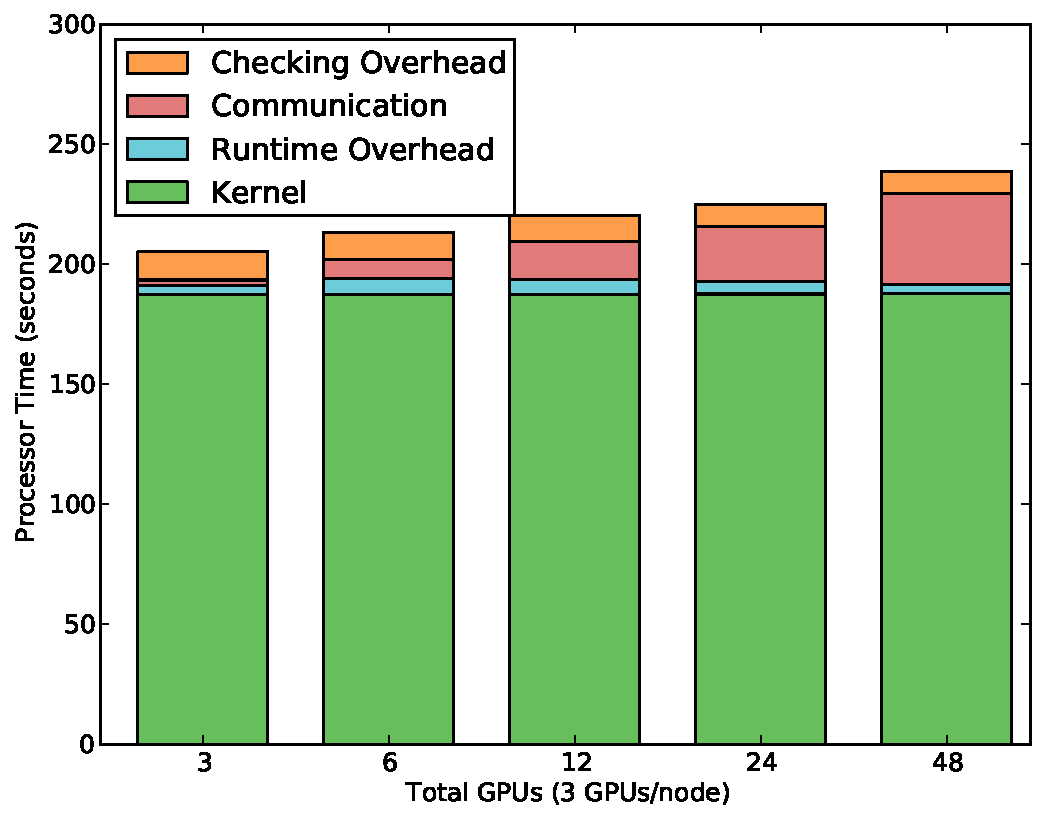
\includegraphics[scale=0.4]{figs/circuit_48_popl.pdf}
%\label{fig:ckt48}
%}
%\subfigure[96 Piece Data Set]
%{
%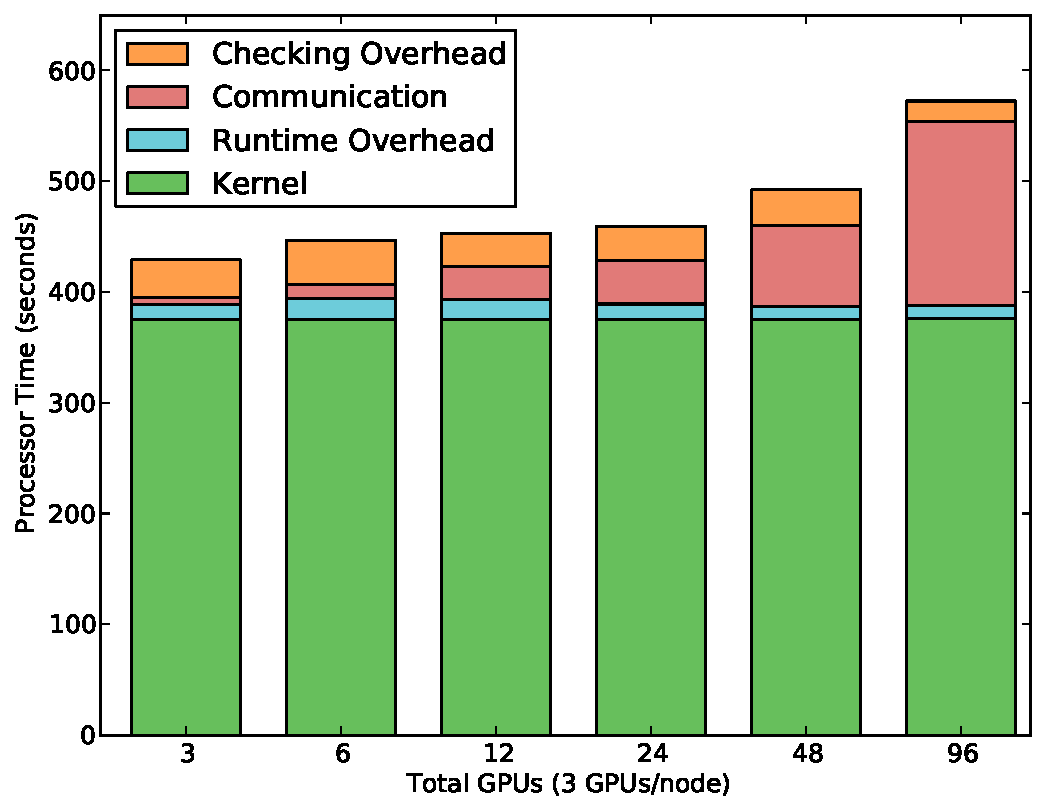
\includegraphics[scale=0.4]{figs/circuit_96_popl.pdf}
%\label{fig:ckt96}
%}
%\caption{Checking overhead of the Circuit simulation.\label{fig:ckt_overhead}}
%\end{figure}

\begin{figure}
\begin{center}
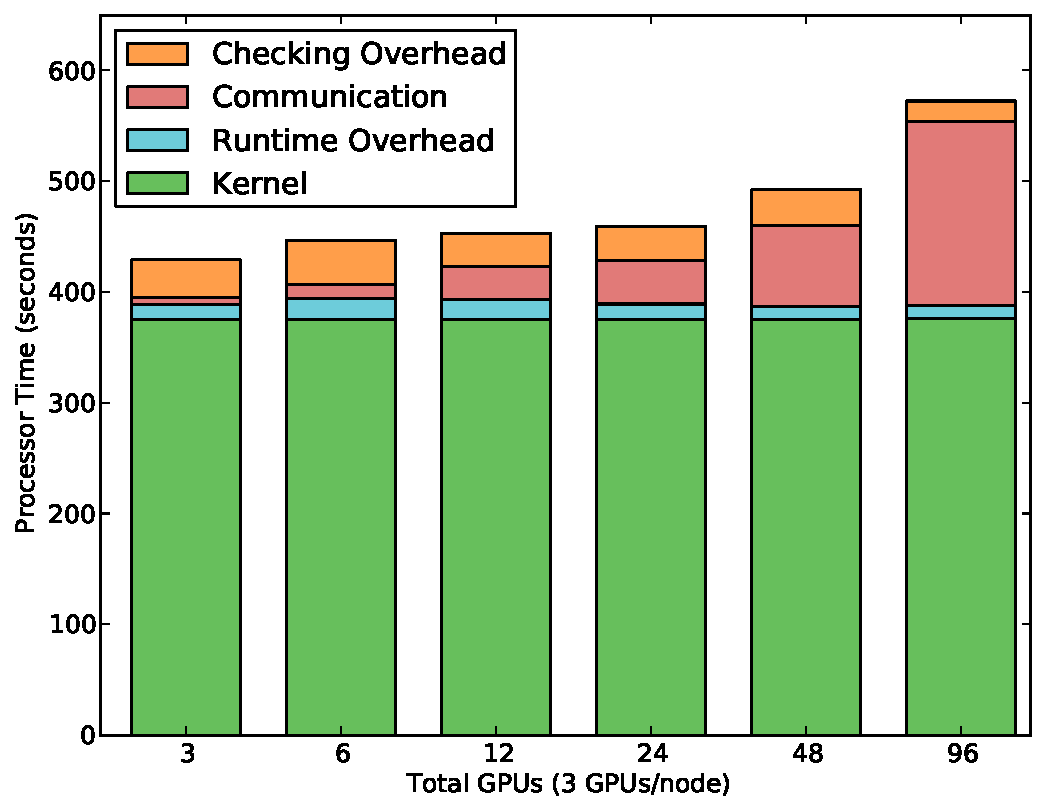
\includegraphics[scale=0.35]{figs/circuit_96_popl.pdf}
\end{center}
\vspace{-2mm}
\caption{Overhead for the Circuit simulation with 96 total pieces.\label{fig:ckt_overhead}}
\vspace{-6mm}
\end{figure}

\begin{figure}
\begin{center}
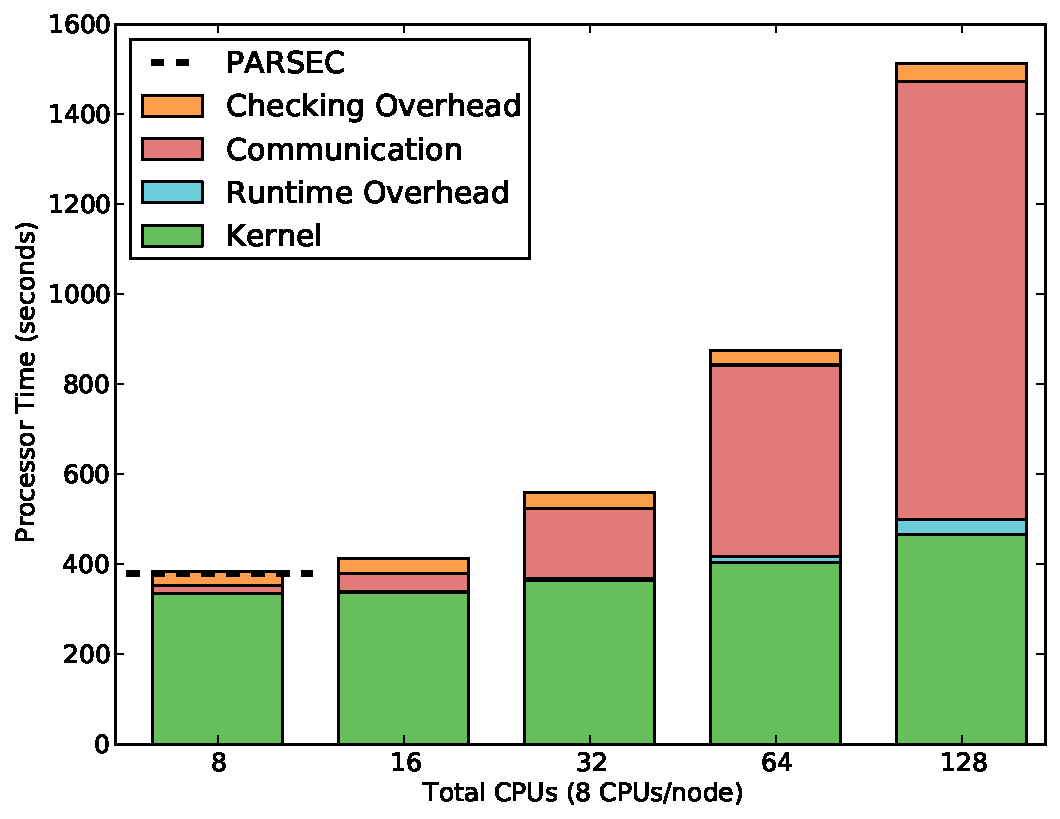
\includegraphics[scale=0.35]{figs/fluid_19200_popl.pdf}
\end{center}
\vspace{-2mm}
\caption{Overhead for the Fluid simulation with 19200 cells.\label{fig:fluid_overhead}}
\vspace{-6mm}
\end{figure}

Figures~\ref{fig:ckt_overhead}, \ref{fig:fluid_overhead}, and \ref{fig:amr_overhead} show 
the total time spent by all CPUs and GPUs in each phase of the application.  The topmost
component of each bar shows the overhead added by the dynamic checks.  In 
each figure the problem size stays the same as the number of processors are increased
(strong scaling).  Figure~\ref{fig:amr_overhead} includes multiple problem sizes to show
how overhead is affected by changing problem size (weak scaling).  For cases where there
is an existing implementation to compare against we have included a dotted line indicating
baseline performance.  In a few cases (Figures~\ref{fig:fluid_overhead} and 
\ref{fig:amr4096}) checking overhead is the difference
between better and worse performance than the baseline.  For an explanation of overall
performance relative to the baseline implementations please refer to \cite{Legion12}.

\begin{figure}
\begin{center}
\subfigure[4096 cells per dimension]
{
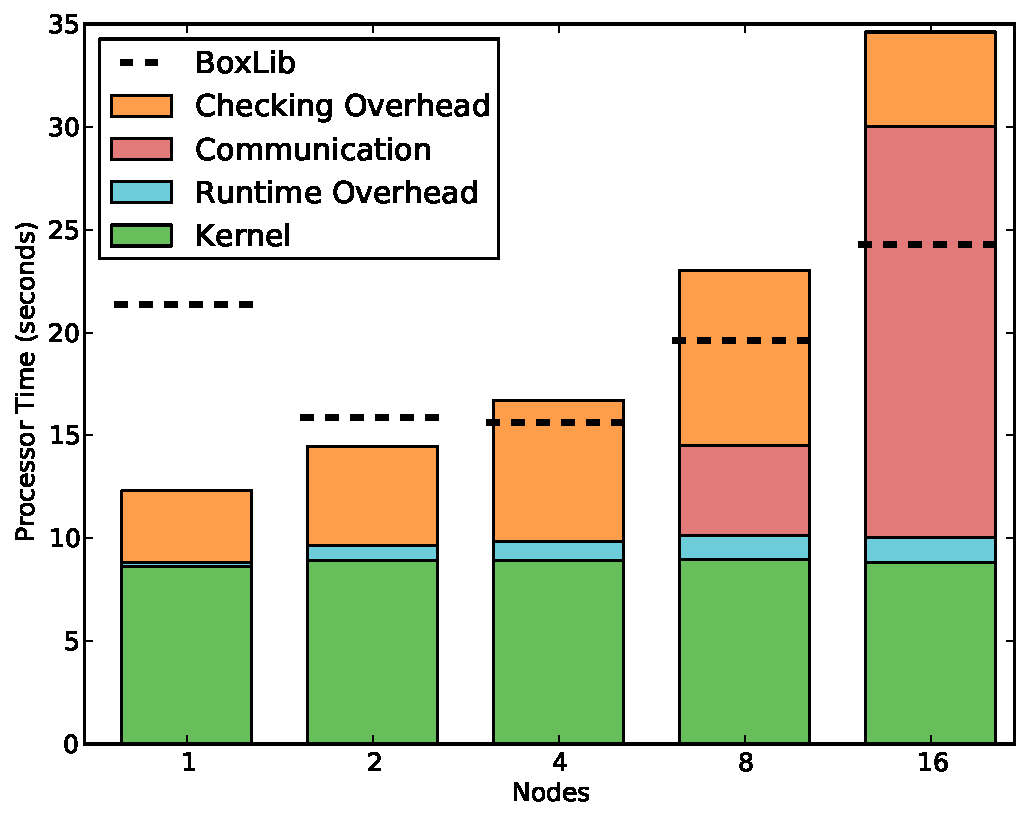
\includegraphics[scale=0.35]{figs/amr_4096_popl.pdf}
\label{fig:amr4096}
}
\subfigure[8192 cells per dimension]
{
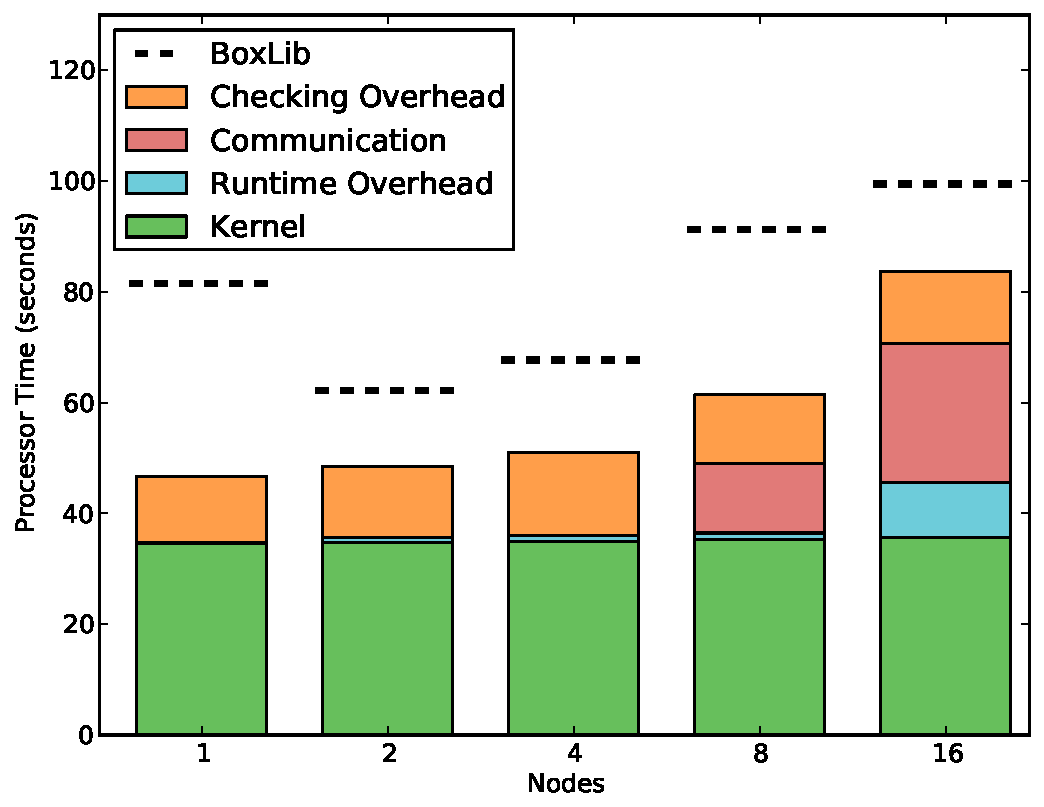
\includegraphics[scale=0.35]{figs/amr_8192_popl.pdf}
\label{fig:amr8192}
}
\subfigure[16384 cells per dimension]
{
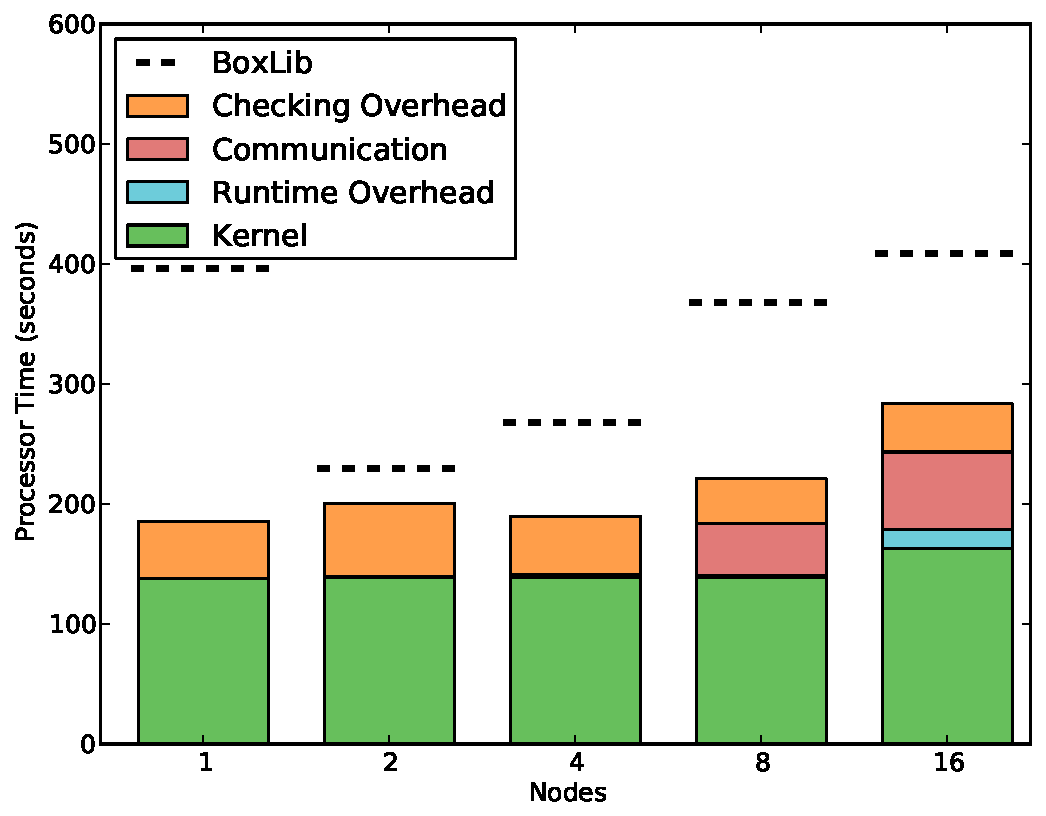
\includegraphics[scale=0.35]{figs/amr_16384_popl.pdf}
\label{fig:amr16384}
}
\end{center}
\vspace{-2mm}
\caption{Overhead for the AMR application.\label{fig:amr_overhead}}
\vspace{-6mm}
\end{figure}

In addition to total processor overhead, we also measured performance gain from eliding checks in 
terms of wall-clock time.  Since most region accesses occur in leaf tasks the checks parallelize 
well.  Wall-clock performance gains from eliding memory checks ranged from 1-10\%, 1-15\%, 
and 2-71\% for Circuit, Fluid, and AMR respectively.  Performance gains for AMR were larger than
the other applications because AMR was already memory bound and the additional checks intensified
memory pressure.  For the GPU kernels in the Circuit application checking required up to 8 additional 
registers per thread.  While the GPU kernels in Circuit where not bound by 
available on-chip memory, kernels that are would be susceptible to extreme performance 
degradation due to the extra registers required for checking.  We also measured the overhead
of the dynamic checks associated with unpack operations but found them to be negligible relative
to the overhead of region access checks.

\subsection{Scalability}
\label{subsec:scalability}
The scalability of Legion derives directly from Theorem~\ref{thm:hiersched}.  This 
theorem makes it safe for the runtime to only perform dependence checks between two
tasks that share the same immediate parent task instead of having to consider all
possible interactions with other tasks anywhere in the system.  Since all tasks that
share the same immediate parent are all created on the node where the parent is executing,
all dependence checks and scheduling decisions can be performed locally with no communication.  
Without this property the runtime would be forced to inform all other processors in the system 
of every task that it launches using expensive broadcasts. 

Figures~\ref{fig:ckt_overhead}, \ref{fig:fluid_overhead}, and \ref{fig:amr_overhead} show that
the overhead of the Legion runtime is always less than 7\% of the total execution time
of the applications.  In some applications communication doesn't scale well, but in these cases communication is
the result of the algorithm being performed and is not caused by runtime communication.
Even in the case of the Circuit application which exhibits quadratic communication, the Legion
runtime is able to achieve a 62.5X speedup on 96 GPUs over a hand-coded single GPU implementation\cite{Legion12}.




\section{Related Work}
\label{sec:related}
Legion is most directly related to Sequoia \cite{Fatahalian06}.  Sequoia is array-based, with
a limited repetoire of ways to partition arrays.  Sequoia is a static language with a single unified hierarchy
of tasks and data; Legion is more dynamic with separate task and region hierarchies.

Deterministic Parallel Java (DPJ) is the only other region-based parallel system of which we are
aware\cite{Bocchino09}.  While there are similarities in the permission system and we have
reused some DPJ notation, there are differences stemming from DPJ's static approach.
Regions in Legion are first-class and can be created, partitioned, packed, and unpacked 
dynamically, allowing programmers to compute data organization at runtime; like Sequoia, DPJ
partition schemes must be statically decided.  Legion allows 
programmers to create multiple partitions of the same region to give different 
views onto the same data, which is not possible in DPJ.  
%DPJ only supports the 
%equivalent to Legion's exclusive and atomic coherence modes \cite{Bocchino11} 
%while Legion provides safe execution even in simultaneous environments.  
There is also a difference in emphasis: DPJ requires shared memory, while Legion 
is designed for distributed heterogenous machines.

Chapel \cite{Chamberlain:Chapel} and X10 \cite{X1005} also provide some Legion-like facilities.
Chapel's domains and X10's places provide the programmer with a 
mechanism for expressing locality, similar to regions in Legion.  However, domains
and places are not used for independence analysis to discover parallelism.
In contrast, Jade uses annotations to describe
data disjointness,  and like Legion leverages the disjointness information
to discover parallelism, but lacks a region system to name and organize unbounded collections of objects \cite{Rinard98}.  

% Unclear to me what subtleties need to be pointed out here and explained
% to properly differentiate our work
Many efforts use static region systems for  memory management (e.g., \cite{Tofte94, Grossman02}).
Our system is more closely affiliated with dynamic region systems used for expressing locality for performance \cite{Gay01}.

%In addition to region languages with static type systems, there have been several
%dynamic region languages.  Cyclone uses both a static type system and dynamic
%region checks to enforce memory safety properties of C programs\cite{Grossman02}.
%Gay and Aiken introduced RC which reference counts regions dynamically and uses
%a static type system to reason about effeciently garbage collecting regions\cite{Gay01}.

There have been many type and effect systems for ownership types
\cite{Boyapati03} including ones that leverage nested regions for describing
relationships \cite{Clarke02,Cameron07}.  However, ownership type and effect systems
are primarily used for reasoning about determinism in object oriented languages and
don't capture the range of disjointness properties that can be specified in Legion.

Reasoning about disjoint heap data is the strong suit of separation logic \cite{Reynolds02}.  
Concurrent separation logic\cite{Brookes04} has been 
used both to parallelize sequential programs\cite{Raza09,Gotsman07} and to provide 
a mechanism for reasoning about independence\cite{Hayman06}.
While we have borrowed some separation logic notation, we ultimately chose to use a 
permissions system as our primary formalism because separation logic does not easily
support reasoning about the interleaving of operations to non-disjoint regions of memory.

% I'm also not sure how much detail to go into here.  DPJ spends a lot of time
% on these papers, but I'm not sure I understand all the details of these papers.
% DPJ also cites Lu06 here, but I'm not sure if we have to
%Type and effect systems have also been used to reason about regions.  FX presented
%the original type and effect system on regions \cite{Lucassen88}, but was restricted 
%to using a finite number of regions and was incapable of describing nested data
%structures.  

% Do we need to enumerate what these disjointness properties are (DPJ does)
%Type and effect systems have also been used in the context of parallelism to discover
%deadlocks and race conditions \cite{Boyapati02,Abadi06,Jacobs08}, but do not present 
%any mechanism for discovering parallelism.

%Still not sure what we want to put here.
% DPJ sites additional separation logic papers but they didn't seem very similar.
% Let me know if you think we should include them as well.





\section{Conclusion}
We have presented Legion, a programming model and
type system for expressing locality and independence
to target heterogeneous, distributed parallel architectures.  
We implemented both a portable high-level and machine 
abstraction low-level runtime to support the Legion 
programming model.  Our implementation of Legion demonstrated
speedups up to 5.9X on a cluster of GPUs.


{
\small
\bibliography{bibliography}
}

\end{document}


